\documentclass[12pt]{article}
\usepackage{graphicx}
\usepackage[utf8]{inputenc}
\usepackage[english]{babel}
\graphicspath{ {images/} }
\usepackage[letterpaper, portrait, lmargin=1.5in, rmargin=1.25in, tmargin=1in, bmargin=1in]{geometry}
\usepackage{color}
\usepackage{setspace}
\usepackage{pdfpages}
\usepackage{booktabs}
\usepackage{dcolumn}
\usepackage[round]{natbib}
\bibliographystyle{unsrtnat}
\newcounter{mysubtable}
\usepackage{amsmath}
\usepackage{caption}
\newcommand\modcounter{%
  \refstepcounter{mysubtable}%
  \renewcommand{\thetable}{\thesection.\arabic{table}\alph{mysubtable}}%
}

\makeatletter
%% The "\@seccntformat" command is an auxiliary command
%% (see pp. 26f. of 'The LaTeX Companion,' 2nd. ed.)
\def\@seccntformat#1{\@ifundefined{#1@cntformat}%
   {\csname the#1\endcsname\quad}  % default
   {\csname #1@cntformat\endcsname}% enable individual control
}
\let\oldappendix\appendix %% save current definition of \appendix
\renewcommand\appendix{%
    \oldappendix
    \newcommand{\section@cntformat}{\appendixname~\thesection\quad}
}
\makeatother

    \usepackage{tabularx}
\usepackage{adjustbox}
%\usepackage{subcaption}
%\DeclareCaptionSubType*[Alph]{table}
%\DeclareCaptionLabelFormat{mystyle}{Table~\bothIfFirst{#1}{ }#2}
%\captionsetup[subtable]{labelformat=mystyle}
\usepackage[toc,page]{appendix}
%\usepackage[flushleft]{threeparttable}


\doublespacing


\title{The External Validity of Experimental Social Preference Games}
\author{Sarah Xu}
\date{April 2018}

\begin{document}

\maketitle


\begin{abstract}

The external validity of social preference games is a growing topic of interest. Many papers have conducted within-subjects experiments, comparing in-lab decisions to real-world decisions. However, the current accumulated evidence is mixed. This research provides a systematic approach: I compared behavior in various social preference games and self-reported measures regarding past social behavior to a natural, far-removed field measure. My results show social preference games do an unsatisfactory job explaining the field behavior. Furthermore, self-reported measures perform just as well, if not better, than the games.

\end{abstract}

\section{Introduction}

The standard economic model assumes individuals\rq \ actions are motivated purely by self-interest. However, from simple observation it is clear that people actually care about the well-being of others: people volunteer, people donate to causes, and social programs exist. If someone is not solely motivated by material self-interest but also cares about the well-being of others, we say that the person has social preferences. The last few decades have seen a strong increase of interest in this topic, with numerous research studies providing evidence of social preferences. %Charness and Rabin 2000; Fehr and Schmidt 1999; Andreoni and Miller 2002; Rabin 1993; Fisman, Jakiela, and Kariv 2014). 
 
When studying social preferences, a common approach is to conduct experiments in a laboratory setting. Participants play experimental games, where they receive monetary incentives aligned with the payoffs of the games. Researchers are able to control and influence prices, information, and actions available to the participants, which allows researchers to rigorously target different aspects of social behavior\footnote{Many papers have identified various aspects of social preferences such as altruism, social welfare, inequality aversion, and reciprocity (e.g., \cite{charness_rabin_2002}; \cite{fehr_schmidt_1999}; \cite{andreoni_miller_2002}; \cite{rabin_1993}; \cite{fisman_jakiela_kariv_2014}).}. Below are common games used to study social preferences: 

\begin{itemize}

\item{Dictator Game}: The player (the dictator) receives an endowment and chooses how to split the amount between themselves and a second player (the receiver).
\item{Ultimatum Game}: Two-player game where the players bargain over a fixed endowment. The first mover (the proposer) divides the sum, and the second mover (the responder) chooses to either accept or reject the offer. If accepted, the proposal is implemented. If rejected, neither player receives any money.
\item{Trust Game}: Two-player game where the first player (the proposer) receives an endowment and proposes how to divide the endowment between themselves and the second mover. The offered amount is multiplied by a factor, and the second player (the responder) decides how much of the multiplied endowment to return to the proposer. 
\item{Public Goods Game}: N-player game where each player receives the same sum of money and simultaneously decides how much to put into a public fund. The total amount in the public fund is multiplied by a factor, and divided evenly amongst the players. \end{itemize}

A big question is the external validity of these social preference games since there are numerous factors that can lead to differences in behaviors in a lab setting versus real-world setting. There are many papers that explore this question, comparing subjects\rq \ lab behavior  to the same subjects\rq \ real-world behavior. \cite{galizzi_navarro-martinez_2017} summarized that about 40\% of reported lab-field correlations and regressions found statistically significant association between lab and field behaviors\footnote{See Galizzi and Navarro-Martinez for their full systematic review and meta-analysis of literature on within-subjects lab-field studies.}. Therefore there is room for further exploration. Similar to previous lab-field experiments, I examined whether in-lab social behavior predicts real-life social behavior. Adopting the experimental design in the study by Galizzi and Navarro-Martinez to provide a systematic approach to the question, I recruited Wesleyan University seniors and recent alumni to play various experimental games: the generalized dictator game, ultimatum game, trust game, and public goods game. I also had participants answer self-reported questions regarding their social behavior as an additional layer to evaluate the predictive ability of the games, and I used donations to Wesleyan University as the field measure.

My results show that social preference games explain little to none of the donations behavior. In fact, the self-reported measures seem to be a better tool than the games. In addition, self-reported measures play a more important role when predicting the field measure. However, further systematic research should be done in order to draw a definite conclusion regarding the external validity of social preference games. 


\section{Literature Review}

There are many papers that study social preferences using experimental games. For example, \cite{forsythe_1994} recruited undergraduate students from the University of Iowa, where they played single dictator and ultimatum games against anonymous opponents. The authors found that, contrary to the subgame perfect Nash equilibrium that both proposers and responders would not send any money, most players in fact gave away proportions of the endowment given to them. \cite{berg_1995} recruited undergraduate students from the University of Minnesota to participate in trust games. 94\% of the proposers sent money, and over one-third of the responders returned an amount greater than what was given to them, showing evidence of trust and reciprocity. \cite{hermann_thoni_gachter_2008} conducted public goods experiments across 16 participant pools, and found that that opportunities for punishment led to varying cooperation levels. These papers are only a few examples from an abundance of literature (with many papers using social preference games not mentioned in the previous section), making it clear that using social preference games has become one of the building blocks of experimental and behavioral economics. 
 
However, laboratory experiments have a disadvantage: they are abstract and remote from realistic situations. Therefore, an important question is the extent to which the experimental games approach to social preferences can be generalized to real world situations. Human behavior may be influenced by a variety of factors that differ between practical and laboratory settings. One issue is that in a laboratory setting, the subject's actions are under the scrutiny of the researcher. \cite{hoffman_1994} found that almost 50\% of their subjects donated at least \$3 (out of a \$10 pie) when playing the dictator game. However, when the authors implemented a ``double-blind'' treatment where both the experimenter and other subjects could not observe the dictator\rq s actions, they found that only 16\% of subjects gave at least \$3. There are other papers that also find that subjects are more prosocial in the lab than they are in the field (e.g., \cite{list_2006}; \cite{gneezy_2004}). Individuals are also influenced heavily on the framing of the situation. For example, in a two-person trust game, \cite{burnham_mccabe_smith_2000} switched between calling the responder ``partner'' and ``opponent'', and found a significant difference in trust and trustworthy behavior. Similarly, \cite{ross_ward_1996} found that simply calling a prisoner's dilemma game either a ``community'' or ``Wall Street'' game wildly varied each treatment group\rq s rates of defection. Studies also find evidence that varying the level of stakes may lead to significantly different behaviors. For example, \cite{carpenter_verhoogen_burks_2005} discovered that increasing the stakes from \$10 to \$100 decreased the median offer in the dictator game from 40\% to 20\%. \cite{slonim_roth_1998} and \cite{parco_rapoport_stein_2002} also found that higher stakes leads to significantly different results than with lower stakes. Interestingly, however, \cite{cherry_frykblom_shogren_2002} found no differences in offers when increasing the stakes from \$10 to \$40. Of course, scrutiny, context, and stakes are only a few factors that can lead to deviations in behavior\footnote{See \cite{levitt_list_2007} for a full discussion of factors, with supporting literature, that may lead to deviations in behavior between laboratory and field settings.}.
 
The fact that varying factors such as scrutiny, context, and stakes can yield significant differences in behavior calls into question the external validity of using experimental games in a laboratory setting to study social preferences. There are a few studies that have examined how subjects\rq \ behavior in a lab setting is compared to the same subjects\rq  \ behavior in a real world situation, and found that in-lab behavior does explain field behavior. \cite{baran_2010} compared MBA alumni donations to their university with their reciprocity behavior when playing the trust game. The authors found that responder behavior predicted university donations. \cite{franzen_pointner_2012} compared behaviors from university students participating in standard dictator games to their actions when receiving a misdirected letter containing money, and found that subjects who showed prosocial behavior in the lab returned the misdirected letters more often than subjects who were selfish in the lab. \cite{englmaier_gebhardt_2011} conducted field experiments where they compared university students\rq \ free riding behavior at the library with free riding behavior in a public goods game, and found statistically significant correlation between field and lab measures. There are also some studies that used non-student subjects: \cite{fehr_leibbrandt_2011} conducted public goods games with Brazilian fishermen, and found that fishermen who were more cooperative in the games were also less likely to exploit the communal fishing grounds. \cite{karlan_2005} compared Peru inhabitants\rq \ trust game behavior to their micro loans repayment behavior, and found correlation between behaviors in the lab game and in the field. 

On the other hand, there are a number of papers that find lab behavior has no explanatory power for field behavior. \cite{goeschl_2015} examined university students\rq \ behavior in two different tasks: a public goods game and their contributions to a task about reducing CO2 emissions. The authors found that behaviors in both tasks were uncorrelated. \cite{hill_gurven_2004} carried out ultimatum and public goods games on Paraguay Ache Indians. They compared the game behaviors to observed food production and sharing patterns to individuals outside the nuclear family and found no significant relationships to lab behavior. \cite{gurven_winking_2008} recruited Tsimane forager-horticulturalists in Bolivia, and compared behavior when playing dictator and ultimatum games to their food-sharing behavior. The authors concluded no relation between the two measures. \cite{voors_2012} studied farmers in Sierra Leone, and compared their behavior in a public goods game to their behavior when asked to contribute to a real community public good. They found no meaningful correlation in behavior between the lab and field measures. 

With other studies finding statistically significant, not statistically significant, and mixed results, the currently accumulated evidence is ambiguous. It is clear that evidence for the external validity of experimental games is weak, justifying that further research is needed. Galizzi and Navarro-Martinez note, however, that the previous studies compared only one social preference game to one specific field measure. The abstract and context-free nature of the games makes it difficult to theoretically map the game to the field measure, and so it is crucial to have a more systematic approach. The authors proceed to carry out their own study where participants answered questions about social behaviors exhibited in the past, played various social preference games, and encountered naturalistic field situations. The field situations included a research assistant asking for help carrying boxes down the stairs, asking to use the participant\rq s phone to make a brief phone call, asking for donations to a children\rq s charity, asking for donations to an environmental charity, or asking for donations to the lab\rq s research fund.  The authors\rq \ overarching conclusion was that behavior when playing the experimental games does a poor job predicting both the survey questions and the field behaviors. They mentioned, however, that more systematic studies are needed in order to draw a definite conclusion.

It is critical to think about why some studies found correlations between lab and field measures and some studies did not, in order to inform the design of my current experiment. While playing the experimental games for the study by Hill and Gurven, participants expressed worry that their choices would make the receiver upset. In particular, the tribal group\rq s culture was heavily focused on community, and was well known for extensive food sharing (which was the field measure the authors used). Perhaps the participants didn\rq t want to risk their choices creating any tension in their community, and getting punished with less food sharing and cooperation. In the studies by Gurven and Winking and Voors et al., participants were also subject to high scrutiny and low anonymity since it was easy for community members to find out the choices each subject made. For my design, an important aspect is that participants played the games in their own time and location. This set-up ensured participants were ensured minimal scrutiny and higher anonymity. 

A criticism of the experimental design by Galizzi and Navarro-Martinez, however, is how the authors executed their field measures: since the setups occur as the participants were exiting their lab session, it is hard to believe that the participants did not connect the encounters to the research lab, especially since they previously answered questions similar in fashion to the current event. This may have led to actions that participants would not have done if they were unaware of the scrutiny. This is called the experimenter demand effect, which is a common problem in experimental design: if participants know their actions are being scrutinized, they may change their behavior towards what constitutes appropriate behavior. Therefore it is better to use a natural, far-removed situation, which is why I used donations to Wesleyan University as the field measure.

\section{Methods}

Each participant was presented with two sets of tasks: (i) incentivized social preference games, and (ii) self-reported questions regarding past social behavior. The field measure used to compare to participants\rq \ lab results is their donations to Wesleyan University.  In addition, I examined which tool, the social preference games, the self-reported measures, or both, is better predict social preferences exhibited in real-world situations.
 
Wesleyan University seniors and recent alumni received an invitation email briefly explaining my research and asking for participation in my study (2,004 emails were provided by Wesleyan University Relations). The entire study was computerized, programmed and implemented using Qualtrics. Online links to both the experimental games and survey questions were included in the email, so those who chose to take part could complete the study remotely. As mentioned in the previous section, the online structure allowed participants to make decisions anonymously and with minimal scrutiny, reducing the risk for exaggerated behavior. Participants received an overview of the two tasks they would complete, and were informed that upon completion of the study, their major, class year, and Wesleyan donations information would be released to me.

In order to incentivize completion of both the games and survey questions, as well as elicit honest game behavior, participants were also informed that completing the entire study made them eligible for a lottery prize. All games used ``tickets" as the experimental currency unit: the total tickets each person earns directly corresponds with how many lottery tickets they own.

I will now explain each of the three main components.

\subsection{Incentivized social preference games}

Those who chose to participate in the study received a unique identifier assigned by Qualtrics. Participants first played four social preference games (in random order): generalized dictator game, ultimatum game, trust game, and public goods game. Before each game, they received detailed instructions along with an example to illustrate how each game worked. For the ultimatum and trust games, each participant had the opportunity to play the roles of both proposer and responder. At the end of the participation deadline, all participants were randomly paired, and ticket payoffs were calculated.

Below are the games each participant played, along with an example for each game: 

\begin{itemize}

\item{Generalized Dictator Game\footnote{The design is based off of the study by Andreoni and Miller.}}:  Each participant, playing as the dictator, played nine different rounds of the generalized dictator game. In each round, participants were given different endowments and prices of giving, and were asked how they would like to divide the endowment with an anonymous, random Player 2. Therefore the budget constraint is given by \(\pi_{s} + p\pi_{o} = \textit{m}\), where \(\pi_{s}\) is how many tickets were kept, \(\pi_{o}\) is how many tickets were given, p is the relative price of giving, and \textit{m} is the endowment. The endowment in each round was either 10, 12, or 15. Every ticket the participant kept was worth either 1, 2, 3, or 4 tickets (hold price), and every ticket given to Player 2 was also worth either 1, 2, 3, or 4 tickets (pass price). Below are the nine sets of endowments and prices of giving used in the study:
\begin{center}
\begin{tabular}{ c c c c c }
\hline \hline
 Budget & Ticket Endowment & Hold Price & Pass Price & Relative Price of Giving \\ 
 \hline
1 & 15 & 1 & 2 & \(\frac{1}{2}\)  \\  
2 & 10 & 1 & 3 & \(\frac{1}{3}\)  \\  
3 & 15 & 2 & 1 & 2 \\  
4 & 12 & 1 & 2 & \(\frac{1}{2}\)  \\  
5 & 10 & 3 & 1 & 3  \\  
6 & 15 & 1 & 1 & 1  \\  
7 & 12 & 2 & 1 & 2 \\  
8 & 10 & 4 & 1 & 4 \\  
9 & 10 & 1 & 4 & \(\frac{1}{4}\)  \\  
\hline \hline \\
\end{tabular}
\end{center}

Participants were given the endowment and hold/pass price for each round, and were presented an interactive slider bar that displayed the different ticket amounts each player could earn. The slider bar ensured choices fulfilled the budget constraint, and eliminated the need to perform calculations by directly showing how many tickets each player would receive.
\subitem \underline{\textit{Example:}} Divide 10 tickets: Hold @ 1 ticket each, Pass @ 3 tickets each. In this example, the endowment is 10 tickets, and the relative price of giving is \(\frac{1}{3}\). That is, however many tickets the player decides to keep is multiplied by 1 (the hold price), and however many tickets given to Player 2 is multiplied by 3 (the pass price). The player is presented a slider bar, ranging from giving 0 tickets to giving 10 tickets, and with each possible offer amount, the player was told the total ticket amounts received by both players in the form (total tickets received, total tickets given). For example, if the player decides to give 4 tickets to Player 2, they would see (6, 12) which means they would receive 6 tickets (10 - 4 = 6) and Player 2 would receive 12 tickets (4 * 3 = 12).

\item{Ultimatum Game}: 
	\begin{itemize}
		\item{Player 1}: Each participant was endowed with 10 tickets, and were told to decide how much of their endowment to send to an anonymous, random responder (Player 2) so that \(\pi_{s} + \pi_{o} = 10\). They were also informed that the responder may or may not reject the proposed allocation: if the allocation is accepted, then the proposal is implemented (Player 1 will receive \(\pi_{s}\) and Player 2 will receive \(\pi_{o}\)), and if the allocation is rejected, neither player receives any tickets.
		\subitem \underline{\textit{Example:}} Suppose the participant chooses to give 3 tickets to Player 2. If Player 2 accepts the proposal, then the participant will receive 7 tickets (10 - 3 = 7) and Player 2 will receive 3 tickets. However, if Player 2 does not like the proposal and rejects the proposition, then both players will receive 0 tickets.
		\item{Player 2}: Each participant was informed that the proposer (Player 1) was given an endowment of 10 tickets. They were presented a list from 0 tickets to 10 tickets (in 1-ticket increments), which represents the different amounts that Player 1 could choose to give them. The participants were instructed to indicate whether they accept or reject each hypothetical proposal, and were told that accepting means they agree to receiving the offered amount, and rejecting means they do not agree and instead both players will receive 0 tickets.
		\subitem \underline{\textit{Example:}} Suppose the participant chooses to reject all offered amounts below 5 tickets, and accept all offered amounts equal to or greater than 5 tickets. If Player 1 chose to offer 3 tickets, then both players will receive 0 tickets. However, if Player 1 chose to offer 6 tickets, then Player 1 will receive 4 tickets (10 - 6 = 4) and the participant will receive 6 tickets.
	\end{itemize}
\item{Trust Game}:
	\begin{itemize}
		\item{Player 1}: Each participant was endowed with 10 tickets. They were prompted to decide how much of their endowment to send to an anonymous, random responder (Player 2) so that \(\pi_{s} + \pi_{o} = 10\). The participants were told that the amount sent over would be multiplied by 3, i.e. Player 2 would receive 3\(\pi_{o}\), and that Player 2 would then decide how many tickets, r \(\leq 3\pi_{o}\), they would like to return. Overall, Player 1 received \(\pi_{s}\)+r tickets and Player 2 received 3\(\pi_{o}\) - r tickets.
		\subitem \underline{\textit{Example:}} If the participant chooses to send 5 tickets, then Player 2 will receive 15 tickets (5 * 3 = 15). Player 2 will then decide how many tickets to return. If Player 2 chooses to 3 tickets, then overall Player 1 will earn 8 tickets (5 + 3 = 8) and Player 2 will earn 12 tickets (15 - 3 = 12).
		\item{Player 2}: Each participant was informed that the proposer (Player 1) received an endowment of 10 tickets. They were then given a list of all ten possible multiplied amounts that Player 1 could have chosen to send, ranging from 3 tickets to 30 tickets in 3-ticket increments. For each possible offered amount, the participants were prompted to enter the number of tickets they would like to return back to the proposer. They were given clear instructions that their input could not exceed what was given to them. For example, if Player 1 gave them a multiplied amount of 15 tickets, then the maximum number of tickets the participant could return is 15 tickets.
		\subitem \underline{\textit{Example:}} Suppose the participant\rq s return scheme is as below: \\
		
\begin{center}
\begin{tabular}{ c c }
\hline \hline
 Possible Offer Amounts (Multiplied) & Tickets Returned \\ 
 \hline
3 & 0  \\  
6 & 1 \\  
9 & 3  \\  
12 & 3  \\  
15 & 5   \\  
18 & 5  \\  
21 & 5 \\  
24 & 5 \\  
27 & 5 \\  
30 & 5 \\  
\hline \hline \\
\end{tabular}
\end{center} 

	where the first column is a list of all possible multiplied amounts that Player 1 could choose to send, and the second column indicates how many tickets the participant would like to return. If Player 1 decided to give 7 tickets to the participant, then the participant will receive a multiplied amount of 21 tickets (7 * 3 = 21). As indicated by the participant\rq s return scheme, the participant chose to return 5 tickets. Thus Player 1 receives 8 tickets (3 + 5 =  8), and the participant receives 16 tickets (21 - 5 = 16).
	\end{itemize}
	
\item{Public Goods Game}: Each participant was given 10 tickets, and told that they would be randomly matched with one other player. They were then prompted to decide how much of their endowment to contribute to a group fund, and that the other player was prompted to do the same task. The total tickets in the group fund was multiplied by 2, and divided evenly between the two players. Therefore each player received the remaining amount of their endowment plus the divided amount from the public fund. The payoff function is given by \( P_{i} = 10 - g_{i} + \sum_{n=1}^{2} g_{n} \) where \(g_{i}\) is the amount that player \textit{i} donated to the fund, and \(\sum_{n=1}^{2}g_{n}\) is the sum of both players\rq \ donations to the public fund\footnote{Note that the players directly receive the total amount donated to the public fund because the multiplied factor, 2, is cancelled by the even split between the two players.}.

\subitem \underline{\textit{Example:}} Suppose the participant chooses to contribute 3 tickets, and the randomly assigned second player chooses to contribute 5 tickets. The total donated amount, \(\sum_{n=1}^{N} g_{n}\) is 8 tickets. Therefore the participant receives: 

\( P_{1} = 10 - g_{1} +  \sum_{n=1}^{2} g_{n} = 10 - 3 + 8 = \) 15 tickets 

and the second player receives: 

\( P_{2} = 10 - g_{2} +  \sum_{n=1}^{2} g_{n} = 10 - 5 + 8 = \) 13 tickets 


\end{itemize}

Appendix C contains all materials (images of each game along with their respective instructions and examples) from the online study.

\subsubsection{Strategy Method}

Since the participants were completing the games at their own availability, they were not randomly matched with other participants until after all data had been collected. As seen with the ultimatum and trust games, which required both a proposer and responder, the responder saw a list of all possible offer amounts and was prompted for their choice for each offer. This is called the strategy method.

There are several reasons why the strategy method is advantageous. It is useful to have all of the responder\rq s potential choices so that payoffs can be determined after the fact. Most importantly, the strategy method gives more information. If players were matched with other players live, then we would only have the responder\rq s response given the proposer\rq s offer. The strategy method, however, provides all returned amounts for all possible donated amounts in the trust game, and provides participants\rq \ minimum accepted amount in the ultimatum game. 

\subsubsection{Payment}

Participants were randomly paired, and ticket payoffs were determined for each game. In each assigned pair, one participant was randomly selected to be Player 1 (i.e. they were the dictator in the generalized dictator game, and proposer in both the ultimatum game and trust game), and the other was Player 2 (i.e. they were the receiver in the generalized dictator game, and the responder in both the ultimatum and trust game). I ran through each game and calculated ticket payoffs for each participant. Since the generalized dictator game consisted of nine rounds, one round was randomly selected. and each participant received the tickets based on their decision for that round. However many total tickets each participant earned from all the games corresponded with the number of tickets they owned in the lottery. Ten tickets were drawn, and each winner received \$100. Winners were emailed instructions on how to receive the prize through direct deposit.

\subsection{Self-reported measures of past social behaviors}

Participants then reported on social behaviors exhibited in the past. The questions are adapted from the Self-Report Altruism (SRA) scale introduced by \cite{rushton_chrisjohn_fekken_1981}. The survey was comprised of 10 items, and participants reported how frequently they have done each item in the past. Participants rated each statement as either ``Never'', ``Once'', ``More than once'', ``Often'', or ``Very often''. Examples include: ``I have donated money at the cash register when buying groceries'', ``I have pointed out a clerk\rq s error (at the supermarket, at a restaurant) in undercharging me'', and ``I have donated instead of sold my clothes/used items''. A full list of the 10 items from the online study is displayed in Appendix D. 

\subsection{Field Measure}

After the participation deadline passed, Wesleyan University Relations provided a dataset that contained each participant\rq s Wesleyan donations information.

Seniors are solicited around once per semester, during senior events. Recent alumni are typically solicited for donations at the end of November / beginning of December, March, and June. Since my online study was released between solicitation cycles for both seniors and recent alumni, and donations information was provided as of January 2018, participants\rq \ donations behavior is not influenced by the experimenter demand effect. 

There are several reasons why I chose to use donations as my field measure. Many behavioral economics papers exploring the relationship between in-lab and field behavior have used donations\footnote{See, e.g., Falk, Meier, and Zehnder; \cite{benz_meier_2006}; Baran et al.}. \cite{falk_2013} justified that donations are an accurate field measure because they do not rely on self-reported responses but on actual decisions. Furthermore, donations are made in private and never made public, and students/alumni are unaware that their actions would be analyzed in a research study. The lack of scrutiny therefore indicates donations should reflect the donors\rq \ genuine altruism. The authors then point out the most important reason for their decision to use donations: all students and alumni are solicited, so everybody has to make the decision about donating.

In addition, donations are a more accurate field measure than creating a scenario at the end of the online session. Donations to Wesleyan University are a far-removed situation, and are not directly related to the study. I previously mentioned that the experimental design by Galizzi and Navarro-Martinez is unsatisfactory since their participants were subject to the experimenter demand effect: because participants encountered the field experiments shortly after completing the lab experiments, it would not be difficult for participants to link the two situations together. Therefore, participants could have acted more pro-socially than they would usually under normal circumstances. In my design, participants\rq \ donations are not affected by their participation in the lab.

\subsubsection{Theoretical Correspondences Between Games and Donations}

All of the social preference games I chose for my study tap into different types of pro-social behaviors that are also related to donating. First, the dictators in the generalized dictator game, proposers in the ultimatum and trust games, responders in the trust game, and players in the public goods game have the option to keep their endowment to themselves, but may also choose to share their endowment with another person. Therefore the actions in these games can be explained by altruism: those who choose to keep their endowment exhibit lower levels of altruism, and those who choose to share their endowment demonstrate higher levels of altruism. Likewise, altruism is the most common representation for donating since the donor chooses to give their income to the university (which in turn benefits future students). 

Proposers\rq \ behaviors in the trust and public goods games indicate their trust levels. In the trust game, since the proposers\rq \ offering gets multiplied by a factor, the proposers may exhibit trust in the responders by sharing their endowment with the hopes of the responders sending back an amount larger than what was given. Similarly in the public goods game, since the total amount donated into the public fund gets multiplied by a factor, players who donate some of their endowment into the public fund may do so with the hopes that the other players will do the same. Correspondingly, donating may also represent trust since donors are trusting that the University will use their donations to benefit future students.

Responders\rq \ actions in the trust game can also be explained by reciprocity: if the proposers decided to share their endowment, the responders then has the opportunity to give back to the proposers. The responders display higher levels of reciprocity if they return some of what was first given to them, and display lower levels of reciprocity if they give back little or nothing. The responders\rq \ action can also be represented by trustworthiness: the proposers may contribute some of their endowment in hopes of the responders returning a larger amount than what was offered. Thus responders who return a larger amount show higher levels of trustworthiness. Equivalently, donations may symbolize reciprocity and trustworthiness since seniors and alumni may donate as thanks for providing them invaluable resources and opportunities.

Players\rq \ responses in all of the games can also correspond with fairness preferences, more specifically inequality aversion. Dictators in the generalized dictator game, proposers in the ultimatum and trust games, responders in the trust game, and players in the public goods game may choose to share their endowment so that the other player will not be left with nothing. Similarly, responders in the ultimatum game may exhibit fairness preferences by rejecting offer amounts of zero (and those who exhibit extreme fairness preferences may reject offer amounts lower than half the endowment). Donations can also symbolize inequality aversion: people may donate because they believe their donations will help students receive opportunities they would not be able to obtain otherwise. In addition, donors are able to target what area their donations can go towards: for example, if the donor targets their donations to Financial Aid, then they are displaying inequality averse preferences.

Lastly, players\rq \ behaviors in the public goods game can also be explained by their cooperation levels. Players may choose to contribute a part of their endowment because they believe the other players are doing the same thing. In the case for donations, people may also exhibit cooperation by donating because the University solicits for donations (i.e. they are cooperating with what the University is asking for), or donating because they believe other seniors and/or alumni are also donating.

	
\subsection{Participants and Sessions}

Wesleyan University Relations provided a random sample of 2,004 emails (334 emails for each class year from 2013 to 2018), and I sent an invitation email in early January 2018 asking for participation in my study. Participants were informed that the study consisted of several experimental games and non-incentivized survey questions, and participation should take no more than 15 minutes.  The deadline for participation was mid-February 2018. A total of 397 people completed the online study. The participants were volunteers who opened the Qualtrics link, provided consent for me to receive their major, class year, and Wesleyan donations data, and completed both the survey questions and social preference games. At the end of the participation deadline, all participants were randomly paired, ticket payoffs were calculated, and 10 winners were randomly selected. The winners were emailed  in the beginning of March 2018 with instructions on how to receive their prizes.

\section{Results}
The results are presented in four distinct sections. I first start by briefly describing the results obtained in the three main elements (social preference games, self-report measure of past social behaviors, and donations). The fourth section will focus on the main research question of the paper: the extent to which the games explain the field behavior. Appendix B contains the variables definition table, and Appendix A contains all of the figures, correlation tables, and regression tables from this section.

\subsection{Social Preference Games}
Since the generalized dictator game consisted of 9 rounds with varying sets of endowments and prices of giving, similar to Andreoni and Miller and \cite{fisman_kariv_markovits_2007}, I assume each participant\rq s giving preferences is a member of the constant elasticity of substitution (CES) utility function.  The CES utility function is written as:\\


\(U_{s} = [\alpha(\pi_{s})^{\rho} + (1-\alpha)(\pi_{o})^{\rho}]^{1/\rho}\) \\


The first parameter, \(\alpha\), measures the relative weight on the payoff for self. Holding \(\rho\) constant, when \(\alpha\)=1, \(U_{s} = \pi_{s}\), i.e. the individual\rq s utility depends only on the amount they keep for themselves. When \(\alpha\)=0, \(U_{s} = \pi_{o}\), i.e. the individual\rq s utility depends only on the amount the other person receives. Therefore as \(\alpha\) approaches 1, the individual exhibits selfish preferences, and as \(\alpha\) approaches 0, the individual exhibits selfless preferences.

The second parameter, \(\rho\), indicates the willingness to trade off payoffs to themselves and the other person in response to price changes. Holding \(\alpha\) constant, \(U_{s} = \alpha\pi_{s} + (1-\alpha)\pi_{o}\) when \(\rho\)=1,  i.e. the individual\rq s utility depends on the sum of the players\rq \ payoffs. This means the individual exhibits perfect substitutes preferences for giving: they will prefer to give their entire endowment to the other player when the price of giving is cheap (p $<$ 1), and they will prefer to keep their entire endowment when the price of giving is expensive (p $>$ 1). These preferences are also called efficiency-minded preferences. As \(\rho \rightarrow -\infty\), \(U_{s} = min(\alpha\pi_{s}, (1-\alpha)\pi_{o})\). That is, the individual\rq s utility equals the minimum payoff between both places, meaning the individual exhibits inequality-averse preferences. These preferences are called Leontief preferences: the individual prefers to split the endowment equally. Lastly, when \(\rho\) = 0, \(U_{s} = A\pi_{s}^{\alpha}\pi_{o}^{1-\alpha}\). In this case, the individual has Cobb-Douglas preferences.\footnote{See \cite{arrow_1961} on how Leontief preferences and Cobb-Douglas preferences are derived from the CES production function.}

Maximizing utility subject to the budget constraint ( \(p_{s}\pi_{s} + p_{o}\pi_{o}=m\) ) yields the CES demand function given by: \\
 

\(\pi_{s}(p,m)=\frac{[\alpha/(1-\alpha)]^{1/(1-\rho)}}{\rho^{-\rho/(\rho-1)}+[\alpha/(1-\alpha)]^{(1/(1-\rho)}}m\) \\

\hspace{14.5mm} \(= \frac{A}{p^{r}+A}m\) \\
 
 \noindent
where \(r=-\rho / (1-\rho) \) and \(A=[\alpha / (1-\alpha)]^{1/(1-\rho)} \). This generates the following individual-level econometric specification for each participant \textit{i}: \\
 
\( \pi^{t}_{s,i} = \frac{A_{i}}{(p^{t}_{i})^{r_{i}} + A_{i}}m^{t}_{i} + \epsilon^{t}_{i}\) \\
 
\noindent
where \textit{i} represents each participant, \textit{t} represents each independent decision-problems in the generalized dictator game, and \( \epsilon^{t}_{i} \) is assumed to be distributed normally with mean zero and variance \(\sigma^{2}_{i}\). For each participant \textit{i}, I used the 9 combinations of \(\pi_{s}\), p, and \textit{m} and generated the estimates  \( \hat{A}_{i} \) and \( \hat{r}_{i} \) using non-linear least squares. From the estimates I retrieved each participant\rq s efficiency level, \( \hat{\rho_{i}}\), which then gave me each participant\rq s sharing propensity, \( \hat{\alpha_{i}} \).

Results for the proposers in the ultimatum game are also represented by the proposers\rq s pass rate, with higher pass rates indicating higher altruism and/or fairness preferences. For example, if the proposer sent 6 tickets to the responder, the pass rate is 0.6. Results for the proposers in the trust game are also represented by the proposer\rq s pass rate (the percentage of the initial endowment passed to the other responder). Higher pass rates indicate higher levels of altruism, fairness preferences, and/or trust. Similarly, outcomes for the players in the public goods games are represented by the proposer\rq s pass rate into the public fund. Thus the larger the amount the player contributes into the public fund signals the higher levels of cooperation the player has. 

Results from the responders in the ultimatum game are represented as the minimum pass rate the responder chooses to accept. Since responders were presented an ascending list of all possible amounts the proposer could choose to send, minimum pass rates were obtained using the switch point where the responders changed from rejecting an offer amount to accepting an offer amount. Lower minimum accepted pass rates indicate lower levels of selfishness and negative reciprocity, whereas higher minimum accepted pass rates indicate higher levels of selfishness and negative reciprocity.

The trust game asks for the responder\rq s return amount given the 10 possible offer amounts from the proposer. For each responder, I regressed their return amount on the offer amount, and retrieved the estimated slope. Thus the results from the responders in the trust game are represented by the estimated slope, which measures the participant\rq s reciprocity, or trustworthiness level. Values closer to one represent more reciprocal behavior, and lower levels closer to zero represent more selfish behavior.\footnote{There may be concern that some participant\rq s may not follow a linear trend. After plotting each participant\rq s return amount in response to the offer amount, I found that with the exception of a few participants, each participant\rq s data points follow a linear slope.}

Figure 1 consists of two panels (Panels A and B) that shows the distribution of parameters, \(\alpha\) and \(\rho\), derived from responses in the generalized dictator game.  The parameter estimates vary dramatically across subjects, implying that preferences for giving are very heterogeneous. Panel A displays a high peak of 21\% at \(\alpha\)=1: a considerable amount of participants displayed extremely selfish preferences. There is a smaller peak of 12\% at \(\alpha\)=0.5, and there are more \(\alpha\) levels above 0.5 than below 0.5. These results show that participants tended to have more selfish preferences. To facilitate presentation of Panel B, participants with very negative \(\rho\) values were combined into the leftmost bar. About 7\% of subjects have perfect substitutes preferences for giving (\(\rho \approx 1\)): these subjects prefer to give their entire endowment to Player 2 when the price of giving is less than one, and keep their entire endowment when the price of giving is greater than one, i.e. efficiency-minded preferences. A little over 20\% of participants demonstrated Leontief preferences (\(\rho\) far below 0), i.e. they prefer splitting the endowment equally, and roughly 15\% of subjects possess Cobb-Douglas preferences (\(\rho \approx 0\)). Many subjects also have intermediate values of \(\rho\): 24\% have preferences for increasing total payoffs (\(0.1 \leq \rho \leq 0.9\)), and almost 20\% have preferences for reducing differences in payoffs between self and others (\(-0.9 \leq \rho \leq 0.9\)).

Figure 2 consists of four panels (Panels C, D, E, and F) which shows the distribution of responses in the ultimatum, trust, and public goods games. Panel C reports a maximum of 42\% of proposers in the ultimatum game who gave half of their endowment to the responders, and there is slightly more emphasis on those who gave contributions lower than half the endowment than contributions higher than half the endowment. These results are in line with the typical patterns in previous literature, which finds that a majority of offers are in the range of 0.25-0.50. Correspondingly, Panel D shows the distribution of the minimum offers that the responder chose to accept. With the exception of one participant who showed extreme negative reciprocity by only accepting an offer of Player 1's entire endowment, everyone accepted an amount less than or equal to half of the endowment. Surprisingly, most participants (27\%) accepted an offer amount of 0 tickets. 

Panel E shows the distribution of contributions the proposers made in the trust game. Pass rates were scattered all across the range from offering none of their endowment to offering all of their endowment. There were two maxima, both around 22\%, at giving half the endowment or the entire endowment. Other contributions that have more than 10\% are proposers who gave 0.3 or 0.4 of the given endowment. This is also broadly in line with typical findings that report average transfers of roughly half of the endowment. Panel F shows that almost half the participants in the public goods game sent their entire endowment into the public fund. The next most popular choice (20\%) was to send half their endowment to the public pool, and only 4\% of participants sent nothing into the public pool. Again, this broadly matches usual results in literature.

Figure 3 contains two panels (Panels G and H) that displays the distribution of reciprocity levels and average repayment rate, respectively, which are derived from responders\rq \ responses in the trust game. Panel G shows that, with the exception of two participants who demonstrated negative reciprocity (perhaps they did not understand the game), reciprocity levels were very heterogenous between 0 and 1. There is a maximum (27\%) at reciprocity levels around 0.5, and a local maximum (14\%) around 0.35. There is also a small local maximum (10\%) at 0, which represents those who did not show any reciprocity. Panel H shows a strong peak of repayment rates of around 0.45, and participants showed slightly stronger preference repaying less than half of what was received versus repaying more than half of what was received. These results are in line with typical patterns found in previous literature, which report average repayment rates of nearly half of the transfer.

Table 1 shows the pairwise correlations (Spearman\rq s \(\rho\)) between the different game outcomes. A large majority of the correlations are statistically significant at the 5\% level (12 out of 15). All of the statistically significant negative correlations involve the \(\alpha\) levels from GDG and the behavior in UG2. The negative correlations for \(\alpha\) reflect that participants who are more selfish (\(\alpha \rightarrow 1\)) are more likely to make smaller contributions in the other games, and the negative correlations for UG2 reflect that participants who accept smaller contributions are more likely to make larger contributions in the other game decisions. Otherwise, decisions in UG1, TG1, TG2, and PGG have positive correlations with one another.
These results show that participants demonstrated consistent behavior in all the games.

\subsection{Self-Reported Measures of Past Social Behaviors}

Total SRA scores were obtained by summing across each participant\rq s responses for the 10 items in the SRA Scale (``Never'' = 0, ``Once'' = 1, ``More than once'' = 2, ``Often'' = 3, ``Very often'' = 4). A higher SRA score indicates higher pro-social behavior. Figure 4 shows the distribution of total scores. There is a wide variety in the total SRA scores obtained, ranging between 20 and 48. Scores are centered around 33 and the shape is symmetric. Panel J displays the distribution of monetary SRA scores, which were obtained by summing across each participant\rq s responses for only the items related to money (items 2, 3, 4, and 7 in Appendix B).  A large majority of the scores are between 9 and 12.

Table 2 contains pairwise correlations (Spearman\rq s \(\rho\)) between the game responses and the SRA scores. I included both total SRA scores (``SRA'') and monetary SRA scores (``SRAmoney''). None of the game results are significantly correlated with total SRA scores, and only the results from the responders in the trust game and players in the public goods game are significantly correlated with the monetary SRA scores. Overall, there is a very weak relationship between the social preference games and self-reported measures. 

\subsection{Donations Behavior}

Figure 5 shows the distribution of Wesleyan donations. Panel I shows that 64\% of the participants have donated to Wesleyan University before, and 36\% have not. Panel J shows the distribution of total donation amounts below \$100, with donations above \$100 aggregated into the rightmost bar. Most of the donation amounts are below \$20 (about 36\%). There are 30 participants who each donated a total amount greater than \$100. All of these larger donations amounts are between \$100 and \$625, with the exception of two very large donations.

\subsection{External Validity of Social Preference Games}
I now turn to the main question of whether the game decisions explain the field behavior. There are two ways that I represented donations behavior: (1) whether the participant has ever donated or not, and (2) the total amount the participant has donated. I included the \(\alpha\) and \(\rho\) parameters from the generalized dictator game, proposers\rq \ pass rates in the ultimatum and trust games (``ultimatum1'' and ``trust1''), responders\rq \ minimum accepted pass rates from the ultimatum game (``ultimatum2''), responders\rq \ reciprocity levels from the trust game (``trust2''), and players\rq \ pass rates in the public goods game (``cooperation'') as the explanatory game variables. I also included total and monetary SRA scores (``SRAtotal'' and ``SRAmoney'') as the explanatory self-reported variables. Appendix B contains the table of variable definitions. 

Table 3 presents twelve logistic regression models using the binary donations representation as the response variable. The first seven columns present each of the game outcomes on their own, and the eighth column includes all of the game variables. The ninth and tenth columns contain SRAtotal and SRAmoney scores on their own, and the last two columns include all of the game outcomes along with the total and monetary SRA scores, respectively. None of the games or SRA results are statistically significant on their own. When both the games and SRA results are used in the regression model, still none of the variables are statistically significant. 

%I then regressed the same explanatory variables on the amount donated. As shown in Figure 5, most donations amounts were fairly small. I therefore used two-limit tobit maximum likelihood, setting the restriction that 0 $\leq$ donations $\leq$ 50.  Table 4 presents the twelve tobit models, presented in the same format as Table 3. The total SRA score is statistically significant at the 10\% level and the monetary SRA score is statistically significant at the 5\% level. Otherwise, none of the social preference games results are statistically significant.
I then used ordinary least squares (OLS) to regress the same explanatory variables on the log of the amount donated. Table 4 presents the twelve linear regression models, presented in the same format as Table 3. Similar to the logistic regression models, none of the game outcomes or SRA scores are statistically significant.

%It is also useful to look at the R$^{2}$ statistic, which measures the proportions of variance explained by the regressors. For both the logistic and tobit regressions, I calculated each model\rq s McFadden\rq s pseudo-R$^{2}$ values\footnote{
%\(R^{2}_{McFadden} = 1 - \frac{log(L_{c})}{log(L_{null})}\)
%where \(L_{c}\) denotes the maximized likelihood for the current fitted model, and \(L_{null}\) denotes the maximized likelihood the model with no predictors.
%}. The values are shown at the bottom of Table 3. The highest value belongs to the model that includes both the games and monetary SRA score. Interestingly, the pseudo-R$^{2}$ value for the model with all of the game variables is lower than the pseudo-R$^{2}$ values for the models that include only the SRA scores. The pseudo-R$^{2}$ values for the tobit regression models are displayed at the bottom of Table 4. The values are very low, and again, the highest value belongs to the model that includes both the games and monetary SRA score. The pseudo-R$^{2}$ value for the model with all of the game variables is higher than the pseudo-R$^{2}$ value for the model that includes only the total SRA score, but is close to the pseudo-R$^{2}$ value for the model that includes only the monetary SRA score. Altogether, these results tell us that self-reported measures are a better tool than even using multiple social preference games when explaining whether people donate or not, multiple social preference games and money-related self-reported measures perform similarly when explaining how much people donate, but the best tool overall is to use both social preference games and self-reported measures. However, all of the R$^{2}$ values are very low - practically zero - so even the ``best'' model explains little to none of the variability of donations behavior.

It is also useful to look at the R$^{2}$ statistic, which measures the proportion of variance explained by the regressors. For the logistic regressions, I calculated each model\rq s McFadden\rq s pseudo-R$^{2}$ values\footnote{
\(R^{2}_{McFadden} = 1 - \frac{log(L_{c})}{log(L_{null})}\)
where \(L_{c}\) denotes the maximized likelihood for the current fitted model, and \(L_{null}\) denotes the maximized likelihood the model with no predictors.
} which are displayed at the bottom of the table. The highest value belongs to the model that includes all of the game outcomes and monetary SRA score (model 12). Interestingly, the pseudo-R$^{2}$ value for the model with all of the game variables is lower than the pseudo-R$^{2}$ values for the models that include only the SRA scores. This suggests that self-reported measures explain the field behavior better than even using multiple social preference games. 

The R$^{2}$ values for the linear regression models are displayed at the bottom of Table 4. The values are very low, and again, the highest value belongs to the model that includes both the games and monetary SRA score (model 12). In contrast to the logistic regression models, the R$^{2}$ value for the model with all of the game variables is larger than the R$^{2}$ values for the models that includes only the total and monetary SRA scores. 

Altogether, these results tell us that self-reported measures are a better tool than even using multiple social preference games when explaining whether people donate or not, and using multiple social preference games is a better than using self-reported measures when explaining how much people donate. The best tool overall, though, is to use both social preference games and self-reported measures. However, all of the R$^{2}$ values are very low - practically zero - so even the ``best'' model explains very little of the variability of donations behavior.

Tables 3 and 4 therefore provide evidence that the social preference games, even when combined with self-reported measures, have little to no power to explain donations behavior. However, this may be because the right combination of variables are not included in the models. I performed best subset selection on both the logistic and linear regression models\footnote{Best subset selection identifies all of the possible regression models derived from all of the possible combinations of the candidate predictors, and determines the model that does the best at meeting some well-defined criteria. In this case, the criteria I used is Mallows\rq \ \(C_{p}\)-statistic, which assesses assess fits when models with different numbers of parameters are being compared.  See \cite{mallows_1973}.}. Since best subset selection fits all possible models to find the best candidate, I included more explanatory variables: I added the responders\rq \ average return outcome from the trust game, and replaced SRAtotal and SRAmoney with each of the ten individual SRA items. I first performed best subset selection for the logistic model, and the chosen model included four of the SRA items were chosen (items 3, 4, 8, and 10). Table 5 displays the best subset logistic regression model. All of the chosen SRA items are statistically significant at the 5\% level. The pseudo-R$^{2}$ value of the model is a lot better than the previous logistic models in Table 3 (almost 8 times larger than the highest value), although it is still pretty low. 

%I then ran best subset selection for the tobit model, and only the \(\rho\) parameter from GDG was selected. Table 6 contains the tobit regression that includes only \(\rho\). However, the variable is not statistically significant, and the psuedo-R$^{2}$ value is not better than the previous tobit models in Table 4. 
Best subset selection on the linear model selected the model that included ultimatum1, trust2, and four of the SRA items (items 3, 4, 5, and 6). Table 6 displays the best subset linear regression model. The third and sixth SRA items are statistically significant at the 10\% level, and the rest of the variables are statistically significant at the 5\% level. The R$^{2}$ statistic is significantly larger than the values in Table 4, but the model still explains only about 15\% of the variability in donations behavior.

%Overall, a few of the SRA items are a slightly better tool than both social preference games and total/monetary SRA scores to explain whether people donate or not, and \(\rho\) was chosen as the best variable to explain the amount people donate. However, the R$^{2}$ values show that each models\rq \ chosen variables still explain little to none of the variability of donations behavior. In addition, some of the game variables in the models have signs that are not expected. First, it makes sense that \(\alpha\) should be negative since higher levels of alpha indicate more selfish behavior. Ultimatum1, trust1, and cooperation should have positive relationships with donations since higher pass rates signal more pro-social preferences. Ultimatum2 is expected to have a negative relationship with donations since higher minimum accepted pass rates signal higher negative reciprocity, and trust2 should have a positive relationship with donations. However, in the logistic model, \(\alpha\), ultimatum1, and ultimatum2 have opposite signs than expected, and in the tobit model, \(\alpha\), ultimatum2, trust1, and trust2 have opposite signs than expected. While these poor results may be discouraging regarding the external validity of social preference games, it is still very interesting as it suggests the social preference games may not generalize field behavior as much as they are expected to.

Overall, a few of the SRA items are a slightly better tool than both social preference games and total/monetary SRA scores to explain whether people donate or not, and a couple of the games (ultimatum and trust games) along with a few of the SRA items were chosen as the best variable to explain the amount people decide to donate. However, each models\rq \ chosen variables still explain only a little of the variability of donations behavior. In addition, some of the game variables in the models have signs that are not expected. First, it makes sense that \(\alpha\) should be negative since higher levels of alpha indicate more selfish behavior. Ultimatum1, trust1, and cooperation should have positive relationships with donations since higher pass rates signal more pro-social preferences. Ultimatum2 is expected to have a negative relationship with donations since higher minimum accepted pass rates signal higher negative reciprocity, and trust2 should have a positive relationship with donations. However, in the logistic models, \(\alpha\), ultimatum1, and ultimatum2 have opposite signs than expected, and in the linear models, \(\alpha\), trust1, and trust2 have opposite signs than expected. Both of these negative results suggest that the external validity of social preference games is pretty weak.

These results also switch us to another interesting topic: although the experimental games and self-reported measures do a poor job explaining donations behavior, perhaps they can still be a useful tool to predict donations behavior. That is, if Wesleyan University wanted to predict donations from upcoming class years, perhaps using social preference games and/or self-reported measures from older class years can help them predict donations behavior.

In predictive modeling, a common approach is to split the data into a training set and testing set. The training set is used to build and train the model. Once the model is ready, the model is tested on the testing set to determine its accuracy and performance. I used the data from the recent alumni participants to create the training set, and used the data from the current seniors to create the testing set. Similar as before, I estimated models for both the binary and continuous representations of donations behavior. The models I estimated include: the logistic/linear regression model, the best-subset logistic/linear regression model, and the least absolute shrinkage and selection operator (lasso) model\footnote{The least absolute shrinkage and selection operator (lasso) is a useful regression analysis method that performs both variable selection and regularization in order to enhance prediction accuracy. The lasso estimate is defined by\\ \\
\( \beta^{lasso}=\mathop\mathrm{argmin}\limits_{\beta} \{ \frac{1}{2} \sum_{i=1}^{N} (y_{i} - \beta_{0} - \sum_{j=1}^{p}x_{ij}\beta _{j})^{2}+\lambda\sum_{j=1}^{p}|\beta _{j}|\} \) \\ \\
where \(\lambda\) is a free parameter set to minimize the out of sample error. Certain coefficients are truncated to be set to zero to effectively choose a simpler model that does not include those coefficients. In other words, lasso regression works like a feature selector that picks out the most important coefficients, i.e. those that are most predictive (and have the lowest p-values). See \cite{tibshirani_1996} for a full introduction on the lasso method.}. To compare how well the models performed, I tested each of the models on the testing set and looked at the mean-squared prediction error (MSPE)\footnote{\(MSPE = E[(g(x_{i}) - \hat{g}(x_{i}))^{2}]\), i.e. the expected value of the squared difference between the fitted values implied by the predictive model \(\hat{g}\) and the values of the (unobservable) model g}, where the smallest MSPE value indicates the best predictive model.

First I estimated logistic regression models on the training set. Table 7 reports each of the models. Each of the estimated models were then tested on the testing set, and the bottom row reports the corresponding MSPE values. The lowest MSPE belongs to the model that includes only the monetary SRA score. Next I performed best subset selection. Table 8 reports the best five models that were chosen, and again, the MSPE values are displayed at the bottom. The model that includes \(\alpha\) and a few of the SRA items (items 3, 4, and 10) has the lowest MSPE. Lastly I used the lasso method, and all of the variables except for \(\alpha\), ultimatum2, and two of the SRA items (items were shrunk to zero. Table 9 shows the lasso penalized logistic model\footnote{Statistical significance tests were based off of the proposed significance test for the lasso by \cite{lockhart_2014}. See \cite{kyung_2010} and Tibshirani for a full discussion on standard errors for lasso predictions.} and its corresponding MSPE value.

I repeated the same steps for the linear models using the log of donation amounts. Table 10 reports the linear regression models, where the lowest MSPE corresponds to the model that includes all of the game variable and monetary SRA score. I ran best subset selection, and Table 11 reports the top five models where the lowest MSPE belongs to the model that contains trust2, ultimatum1, and four of the SRA items (items 3, 4, 5, 6, and 10) . Finally, the lasso method truncated most of the variables to zero, leaving out two SRA items (items 4 and 6). Table 12 shows the lasso penalized linear model with its MSPE value.

Below are tables that report each predictive model\rq s MSPE values:


\begin{center}
\begin{adjustbox}{width=\textwidth}
\begin{tabular}{ c | c | c }
\hline \hline
Logistic model & Best subset logistic model & Lasso penalized logistic model \\ 
\hline
\small donated = \(\alpha\) + \(\rho\) + ultimatum1 +  ultimatum2 + & donated = \(\alpha\) + SRA3 + SRA4 + SRA10 & donated = \(\alpha\) + ultimatum2 + SRA3 + SRA4 \\
\small trust1+ trust2 + cooperation + SRAmoney & & \\
 \hline
 0.39818 & 0.38435 & 0.39048 \\  
 \hline \hline
\end{tabular}
\end{adjustbox}
\end{center}
 
 
 
\begin{center}
\begin{adjustbox}{width=\textwidth}
\begin{tabular}{ c | c | c }
\hline \hline
Linear model & Best subset linear model & Lasso penalized linear model \\
\hline
log(donations) = \(\alpha\) + \(\rho\) + ultimatum1 +  ultimatum2 + & log(donations) = trust2 + ultimatum1 + SRA3 + & log(donations) = SRA4 + SRA6 \\
\small trust1+ trust2 + cooperation + SRAmoney & SRA4 + SRA5 + SRA6 + SRA10 & \\
\hline
7.05559 & 6.36137 & 2.72603 \\
\hline \hline
\end{tabular}
\end{adjustbox}
\end{center}

The first table shows that the best subset model containing \(\alpha\) from the generalized dictator game and three SRA items is the most accurate model for predicting whether people will donate or not. Something to note, however, is that the difference between the MSPE values is very small: whether all of the social preference games are used or only a couple are used, the prediction performances are similar.

The second table shows that the lasso penalized model containing the two SRA items is the best-performing model for predicting donation amounts.

\section{Discussion and Conclusion}

Currently, the accumulated literature exploring the external validity of social preference games have mixed results. My thesis provides a systematic approach to this topic where I elicited decisions in four experimental social preference games along with self-reported social behaviors performed in the past. Most importantly, I used a natural field measure that is far-removed from my study.

The overall conclusion is that the social preference games do a poor job explaining the field behavior. In fact, the self-reported measures explain donations behavior similarly, if not better, to the games. It is particularly striking that they do not seem to explain to any significant extent any of the behaviors observed in the field. These poor results are still very interesting, however, because it suggests that social preference games may not generalize as much as it is anticipated to. Social preference games are thought to at least generally indicate individuals\rq pro-social behavior. With the results from my research, however, this doesn\rq t seem to be the case. 

Self-reported measures also played a more prominent role than the games in predicting donations behavior. For both the logistic and linear case, a few game parameters were selected in some models, but the SRA items represented a majority of the explanatory variables in each model.

Altogether, self-reported measures perform just as well (if not better) than social preference games in both explaining and predicting donations behavior. This conclusion has a potential policy implication from a research perspective. Experimental games require a lot of resources - not only is it expensive paying participants for attending the lab session and providing money aligned with the payoffs of the games, but it also takes a lot of time to program the experimental games. Therefore perhaps eliminating experimental games in favor of survey questions is more efficient.

However, this is just the beginning of a systematic approach to uncovering the external validity of experimental social preference games. There are a few things that further research can include. First, both Galizzi and Navarro-Martinez and my study used university (recent) students who self-selected into the experiments. It would be beneficial to use a different participant pool, since our subjects could be inherently different than the general population\footnote{See Levitt and List for a discussion on student participants}. Further research should also use more field measures. Galizzi and Navarro-Martinez created five field situations. However, their subjects were likely influenced by the experimenter demand effect. On the other hand, my study included only one field measure, but the measure was far removed. Therefore further research should incorporate more field measures that can be theoretically mapped to various behavioral constructs, but also far removed from the study itself.

Finally, this research may potentially spark interest into future studies into the external validity of other behavioral economics topics where lab experiments are also commonly used. For example, using experiments to study risk preferences and time preferences is common, so it would be intriguing to adopt a systemic approach to explore whether in-lab behavior is correlated to field measures.

\newpage
\bibliography{mybibliography}
%\bibliographystyle{apalike}

% \newpage
%\begin{thebibliography}{9}
%
%\bibitem{AndreoniMiller}
%Andreoni, J., and Miller, J.H. (2002).
%\textit{Giving according to GARP: An experimental test of the consistency of preferences for altruism}.
%Econometrica, 70, 737-53.
%
%\bibitem{Baran}
%Baran, N.M., Sapienza, P., and Zingales, L. (2010).
%\textit{Can we infer social preferences from the lab? Evidence from the trust game}.
%NBER Working Paper 15654.
%
%\bibitem{Benz}
%Benz, M., and Meier, S. (2006).
%\textit{Do people behave in experiments as in the field? Evidence from donations}.
%Experimental Economics, 11, 268-81.
%
%\bibitem{Berg}
%Berg, J., Dickhaut, J.W., and McCabe, K.A. (1995).
%\textit{Trust, reciprocity, and social history}.
%Games and Economic Behavior, 90, 166-93.
%
%\bibitem{Burnham}
%Burnham, T., McCabe, K., Smith, V. (2000).
%\textit{Friend-or-foe intentionality priming in an extensive form trust game}.
%Journal of Economic Behavior \& Organization, 43, 57-73.
%
%\bibitem{Carpenter}
%Carpenter, J.P., Verhoogen, E., and Burks, S. (2005).
%\textit{The effect of stakes in distribution experiments}.
%Economics Letters, 86, 393-98.
%
%\bibitem{CharnessRabin}
%Charness, G., and Rabin, M. (2002).
%\textit{Understanding social preferences with simple tests}.
%Quarterly Journal of Economics, 117, 817-69.
%
%\bibitem{Cherry}
%Cherry, T., Fykblom, P., and Shogren, J. (2002).
%\textit{Hardnose the Dictator}.
%American Economic Review, 92(4): 1218-21.
%
%\bibitem{Englmaier}
%Englmaier, F., and Gebhardt, G. (2010)
%\textit{Free-riding in the lab and in the field}.
%CESifo Working Paper No. 3612.
%
%\bibitem{FehrLeibbrandt}
%Fehr, E., and Leibbrandt, A. (2011)
%\textit{A field study on cooperativeness and impatience in the Tragedy of the Commons}.
%Journal of Public Economics, 95, 1144-55.
%
%\bibitem{FehrSchmidt}
%Fehr, E., and Schmidt, K. (1999).
%\textit{A theory of fairness, competition, and cooperation}.
%Quarterly Journal of Economics, 114, 173-68.
%
%\bibitem{Fisman1}
%Fisman, R., Jakiela, P., and Kariv, S. (2014).
%\textit{The distributional preferences of Americans}.
%NBER Working Paper.
%
%\bibitem{Fisman2}
%Fisman, R., Kariv, S., and Markovits, D. (2007).
%\textit{Individual Preferences for Giving}.
%American Economic Review, 97(5): 1858-76.
%
%\bibitem{Franzen}
%Franzen, A., and Pointner, S. (2013)
%\textit{The external validity of giving in the dictator game: A field experiment using the misdirected letter technique}.
%Experimental Economics, 16, 155-69.
%
%\bibitem{Galizzi}
%Galizzi, M., and Navarro-Martinez, D. (2017).
%\textit{On the external validity of social preference games: a systematic lab-field study}.
%Management Science.
%
%\bibitem{Gintis}
%Gintis, H. (2000).
%\textit{Strong reciprocity and human sociality}.
%Journal of Theoretical Biology, 206, 169-79.
%
%\bibitem{Gneezy}
%Gneezy, U., Haruvy, E., and Yafe, H. (2004).
%\textit{The inefficiency of splitting the bill: A lesson in institutional design}.
%The Economic Journal, 114(495), 265-80.
%
%\bibitem{Goeschl}
%Goeschl, T., Kettner, S.E., Lohse, J., and Schwieren, C. (2015)
%\textit{What do we learn from public good games about voluntary climate action? Evidence from an artefactual field experiment}.
%University of Heidelberg, Department of Economics Discussion Paper 595.
%
%\bibitem{GurvenWinking}
%Gurven, M., Winking, J. (2008).
%\textit{Collective action in action: prosocial behavior in and out of the laboratory}.
%American Anthropologist, 110(2), 179-190. 
%
%
%\bibitem{Henrich}
%Henrich, J., et al. (2005).
%\textit{``Economic Man'' in Cross-Cultural Perspective: Ethnography and Experiments from 15 Small-Scale Societies}.
%Behavioral and Brain Sciences. 28(6): 795?815.
%
%\bibitem{Hermann}
%Hermann, B., Thoni, C., and Gachter, S. (2008).
%\textit{Anti-social punishment across societies}.
%Science, 319, 1362-67.
%
%\bibitem{HillGurven}
%Hill, K., and Gurven, M. (2004)
%\textit{Economic experiments to examine fairness and cooperation among the Ache Indians of Paraguay}.
%In J. Henrich, R. Boyd, S. Bowles, C. Camerer, E. Fehr, and H. Gintis (Eds.),
%Foundations of Human Sociality: Economic Experiments and Ethnographic Evidence from Fifteen Small-Scale Societies. Oxford University Press.
%
%\bibitem{Hoffman}
%Hoffman, E., McCabe, K., Shachat, K., and Smith, V. (1994).
%\textit{Preferences, property rights, and anonymity in bargaining games}.
%Games and Economic Behavior, 7(3): 346-80.
%
%\bibitem{Karlan}
%Karlan, D.S. (2005).
%\textit{Using experimental economics to measure social capital and predict financial decisions}.
%American Economic Review, 95, 1688-99.
%
%\bibitem{Levitt}
%Levitt, S., and List, J. (2007)
%\textit{What do laboratory experiments measuring social preferences reveal about the real world?}.
%Journal of Economic Perspectives, 21(2), 153-74.
%
%
%\bibitem{List}
%List, John. 2006.
%\textit{The behavioralist meets the market: measuring social preferences and reputation effects in actual transactions}.
%Journal of Political Economy, 114(51), 1-37.
%
%
%\bibitem{Parco}
%Parco, J., Rapoport, A., and Stein, W. (2002).
%\textit{Effects of financial incentives on the breakdown of mutual trust}.
%Psychological Science.
%
%\bibitem{Rabin}
%Rabin, M. (1993).
%\textit{Incorporating fairness into game theory and economics}.
%The American Economic Review, 83, 1281-1302.
%
%\bibitem{Ross}
%Ross, L., and Ward, A. (1996).
%\textit{Naive realism in everyday life: Implications for social conflict and misunderstanding}.
%Values and Knowledge, 103-35.
%
%\bibitem{Rushton}
%Rushton, J.P., Chrisjohn, R.D., and Fekken, G.C. (1981).
%\textit{The altruistic personality and the self-report altruism scale}.
%Personality and Individual Differences, 2, 293-302.
%
%\bibitem{Slonim}
%Slonim, R., and Roth, A. (1998).
%\textit{Learning in high stakes ultimatum games: An experiment in the Slovak Republic}.
%Econometrica, 66, 569-96.
%
%
%\bibitem{Voors}
%Voors, M., Turley, T., Kontoleon, A., Bulte, E., and List, J.A. (2012).
%\textit{Exploring whether behavior in context-free experiments is predictive of behavior in the field: Evidence from lab and field experiments in rural Sierra Leone}.
%Economic Letters, 114, 308-311.
%
%
%\end{thebibliography}
%
\newpage

\appendix

\section{Computerized Social Preference Games} \label{app:a} 
\vspace{8mm} 
\noindent Generalized Dictator Game (GDD) \\ \\
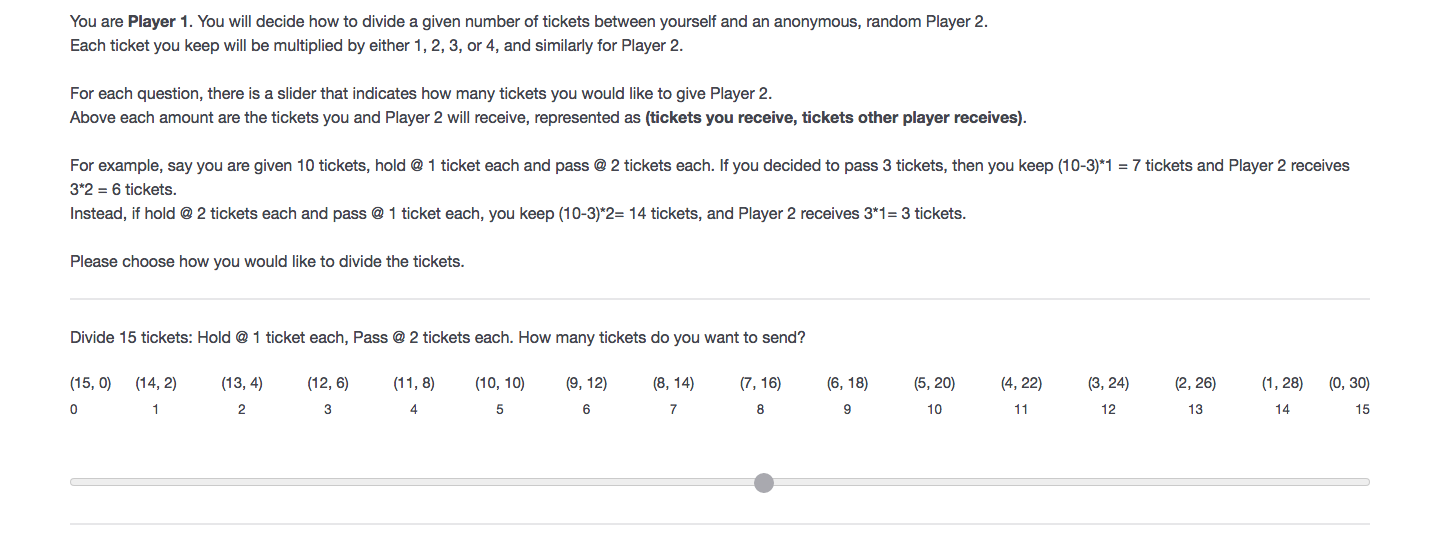
\includegraphics[scale=0.35]{gendict1}\\
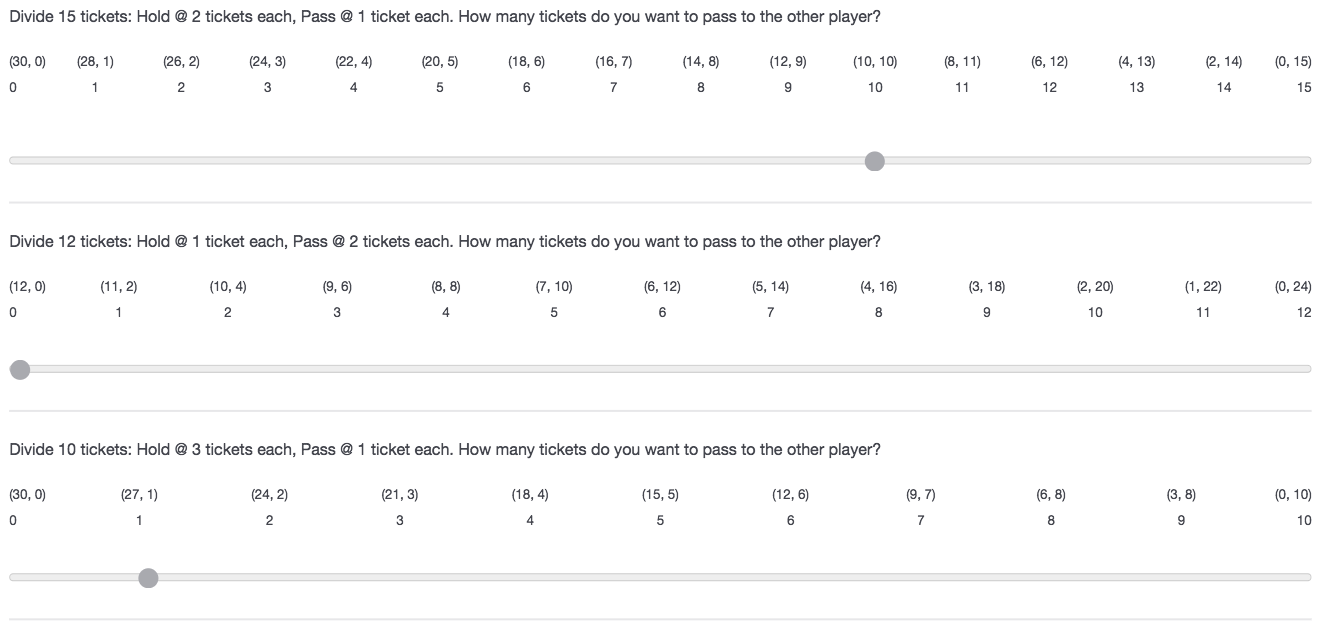
\includegraphics[scale=0.35]{gendict2}\\
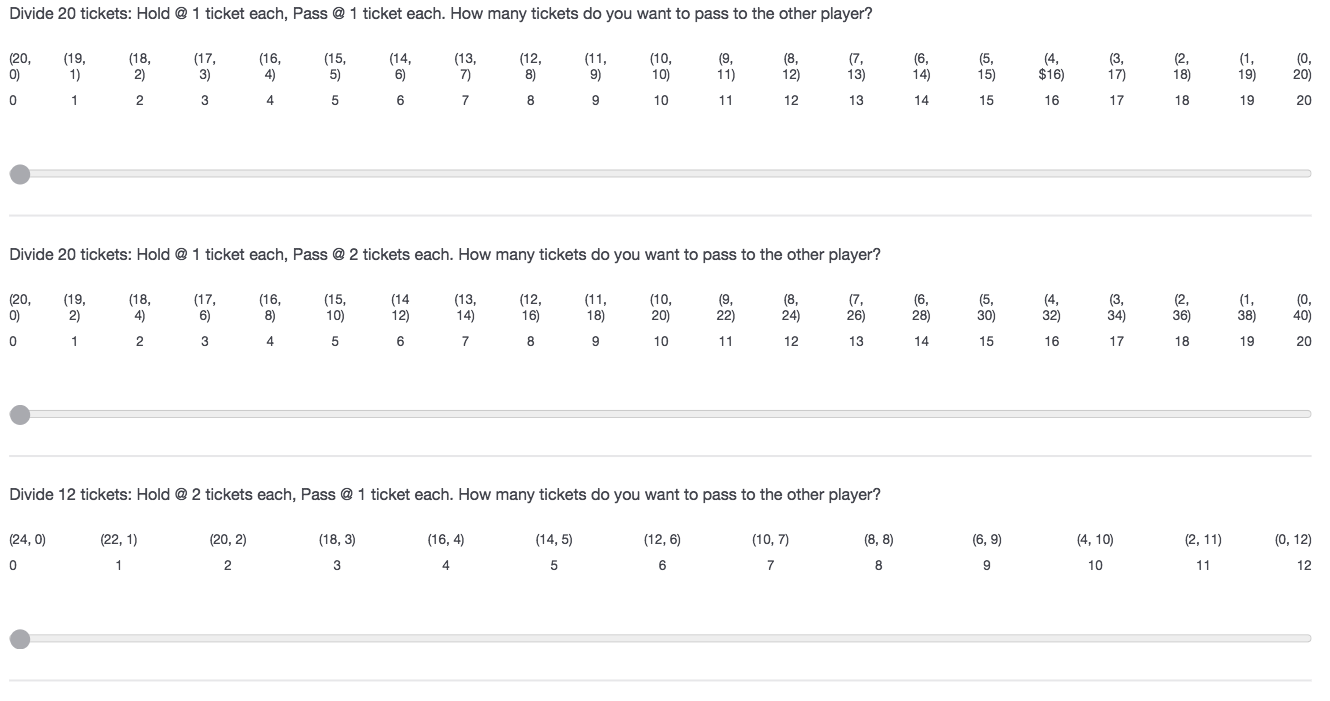
\includegraphics[scale=0.35]{gendict3}\\
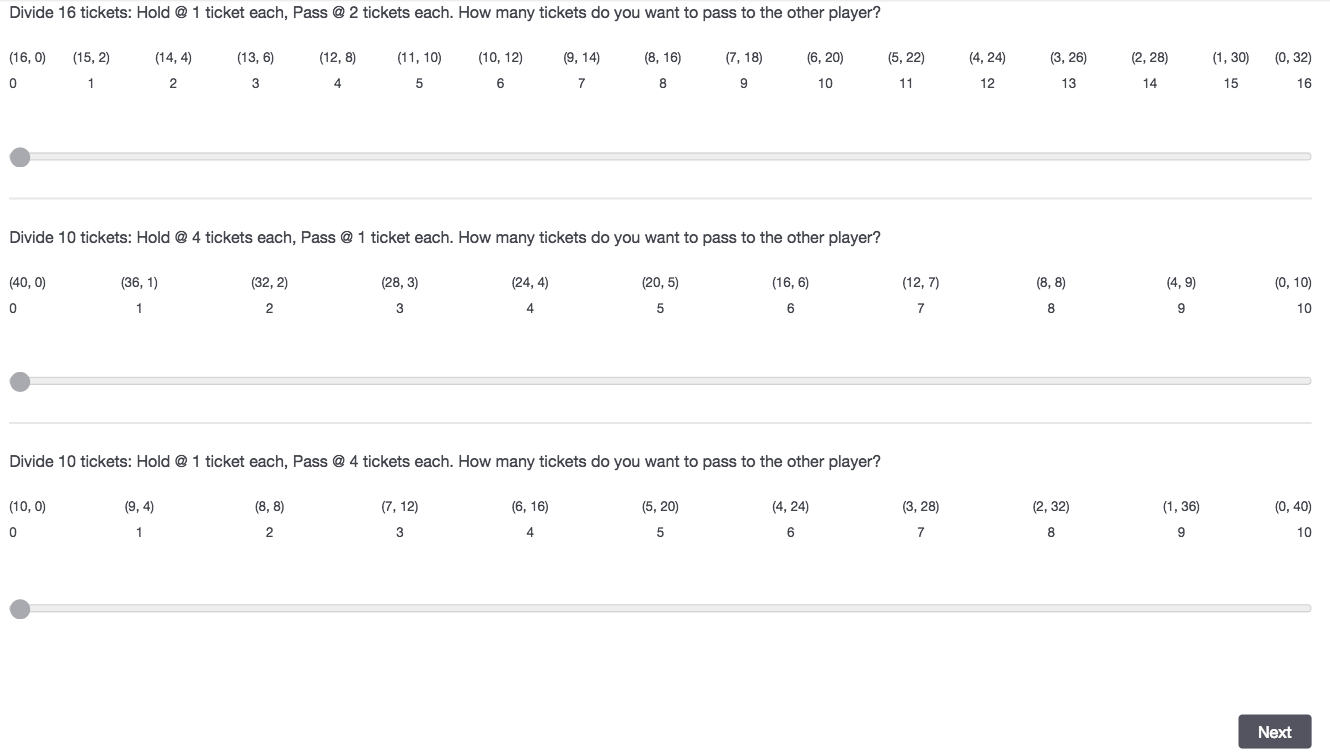
\includegraphics[scale=0.35]{gendict4}\\ \\
\noindent Ultimatum Game Player 1 (UG1) \\ \\ 
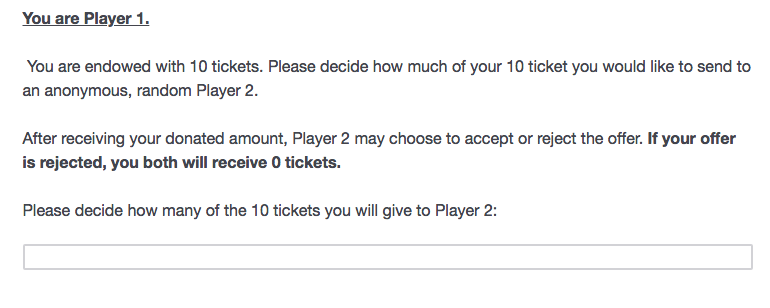
\includegraphics[scale=0.35]{ultimatum1} \\ \\
\noindent Ultimatum Game Player 2 (UG2) \\ \\
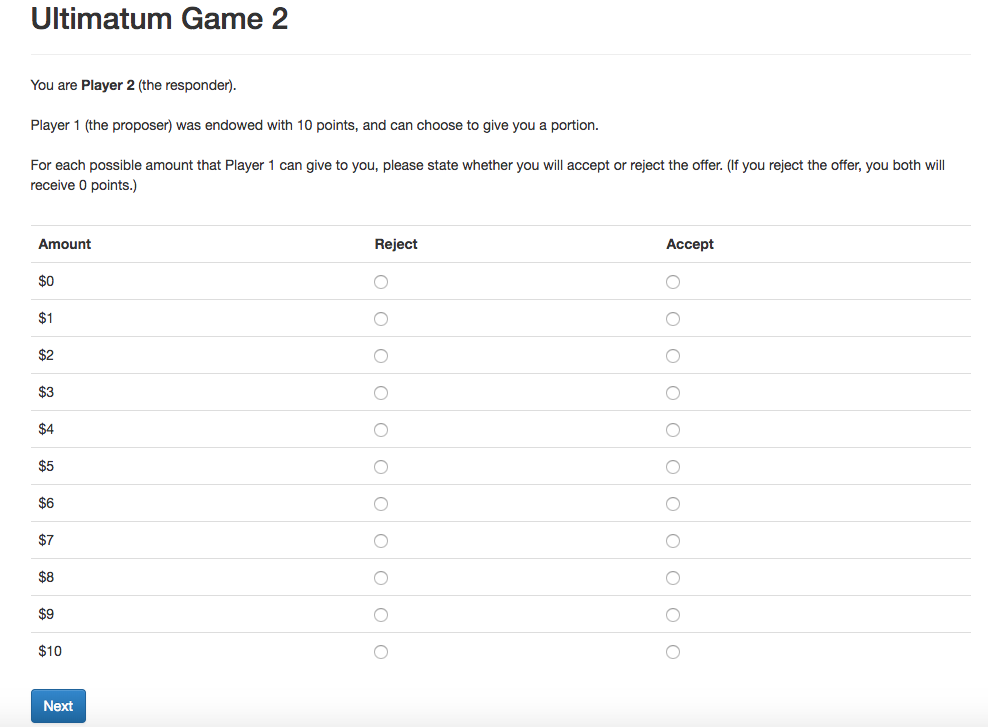
\includegraphics[scale=0.35]{ultimatum2} \\
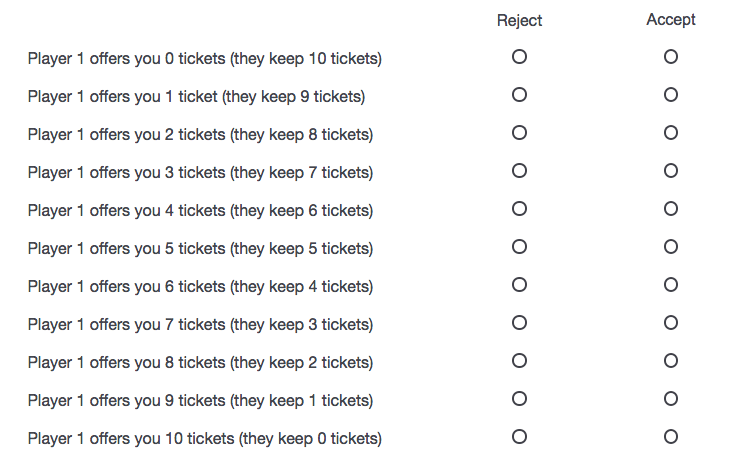
\includegraphics[scale=0.35]{ultimatum3} \\ \\
\noindent Trust Game Player 1 (TG1) \\ \\
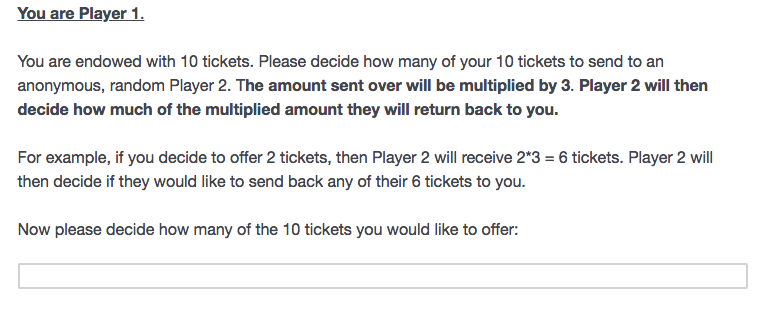
\includegraphics[scale=0.35]{trust1} \\ \\
\noindent Trust Game Player 2 (TG2) \\ \\
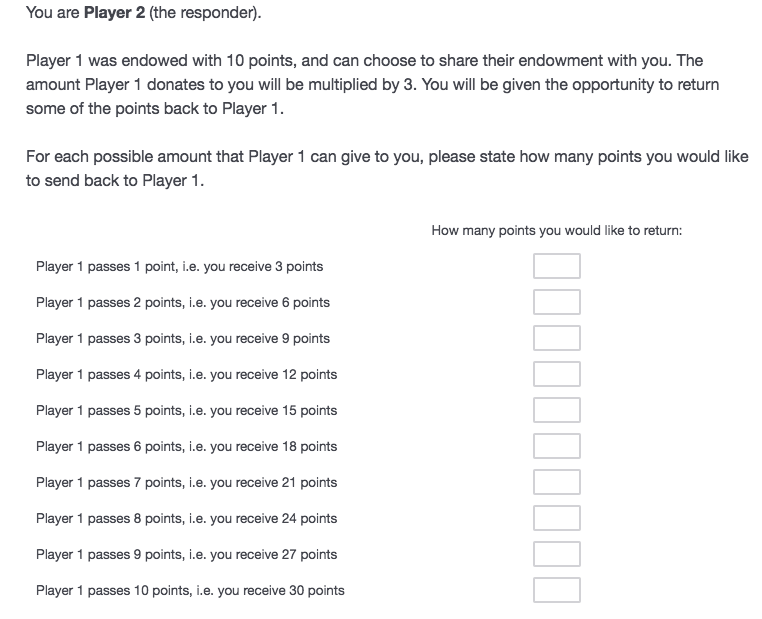
\includegraphics[scale=0.35]{trust2} \\
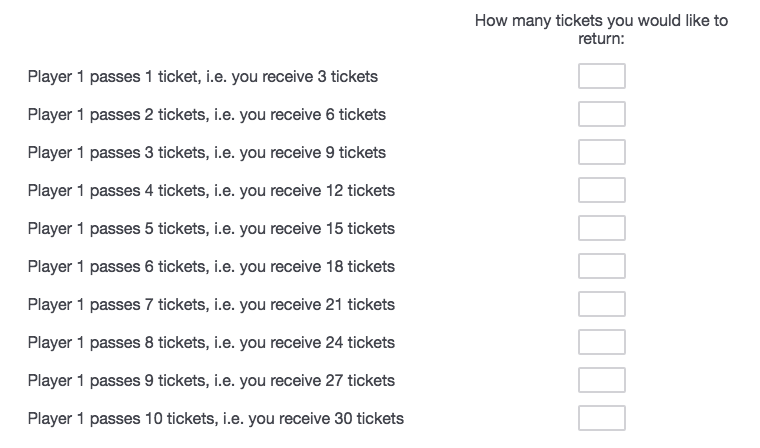
\includegraphics[scale=0.35]{trust3} \\ \\
\noindent Public Goods Game (PGG) \\ \\
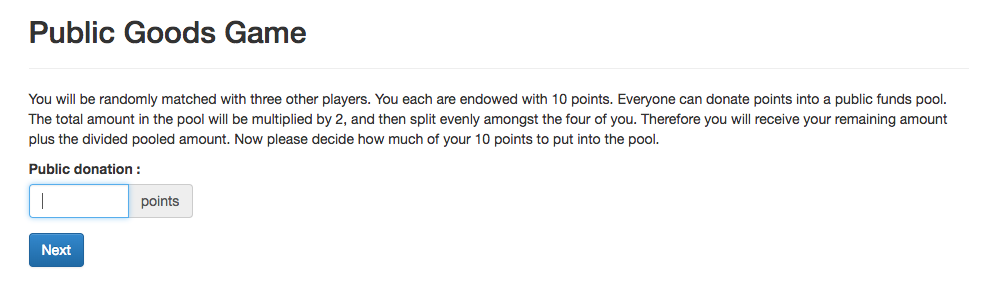
\includegraphics[scale=0.35]{public} \\



\section{Self-Report Altruism (SRA) Questions List} \label{app:b}


\begin{tabular}{ | p{12cm} | }
\hline
%\multicolumn{1}{|c|}{SRA Questions List} \\
%\hline
1. I have allowed someone to go ahead of me in line.\\
\hline
2. I have donated money at the cash register when buying groceries.*\\
\hline
3. I have given money to a stranger (or an acquaintance I don\rq t know too well) in need.*\\ 
\hline
4. I have donated to a charity.*\\
\hline
5. I have done volunteer work for a charity/organization.\\
\hline
6. I have delayed an elevator/held door open for stranger(s).\\
\hline
7.  I have pointed out a clerk\rq s error (at a supermarket, restaurant) in undercharging me.*\\
\hline
8. I have gone out of my way to meet with someone to help them with a task (e.g. help proofread their paper, listen to their presentation, etc). \\
\hline
9. I have offered my seat on a bus/train to a stranger who was standing.\\
\hline
10. I have helped an acquaintance with moving in/ moving out of their dorm/apartment/house.\\
\hline
\end{tabular} \\
\small Note: * indicates SRA item is related to money. \\ \\

\section{Variables Definition Table} \label{app:c}

\begin{center}
\begin{tabular}{ |c|c| } 
 \hline
 Alpha & Player\rq s \(\alpha\) level derived from the generalized dictator game \\ 
 \hline
  Rho & Player\rq s \(\rho\) level derived from the generalized dictator game \\ 
 \hline
 Ultimatum1 & Player 1\rq s pass rate in ultimatum game \\ 
 \hline
 Ultimatum2 & Player 2\rq s minimum pass rate accepted in ultimatum game  \\ 
 \hline
 Trust1 & Player 1\rq s pass rate in trust game \\ 
 \hline
 Trust2 & Player 2\rq s reciprocity level in trust game \\ 
 \hline
 Cooperation & Player\rq s pass rate into public pool in public goods game  \\ 
 \hline
 SRAmoney & Player\rq s monetary SRA score \\ 
 \hline
 SRAtotal & Player\rq s total SRA score \\ 
\hline
\end{tabular}
\end{center}




\section{Figures and Tables} \label{app:d}

\noindent Figure 1: Distribution of CES parameters from GDG \\ \\
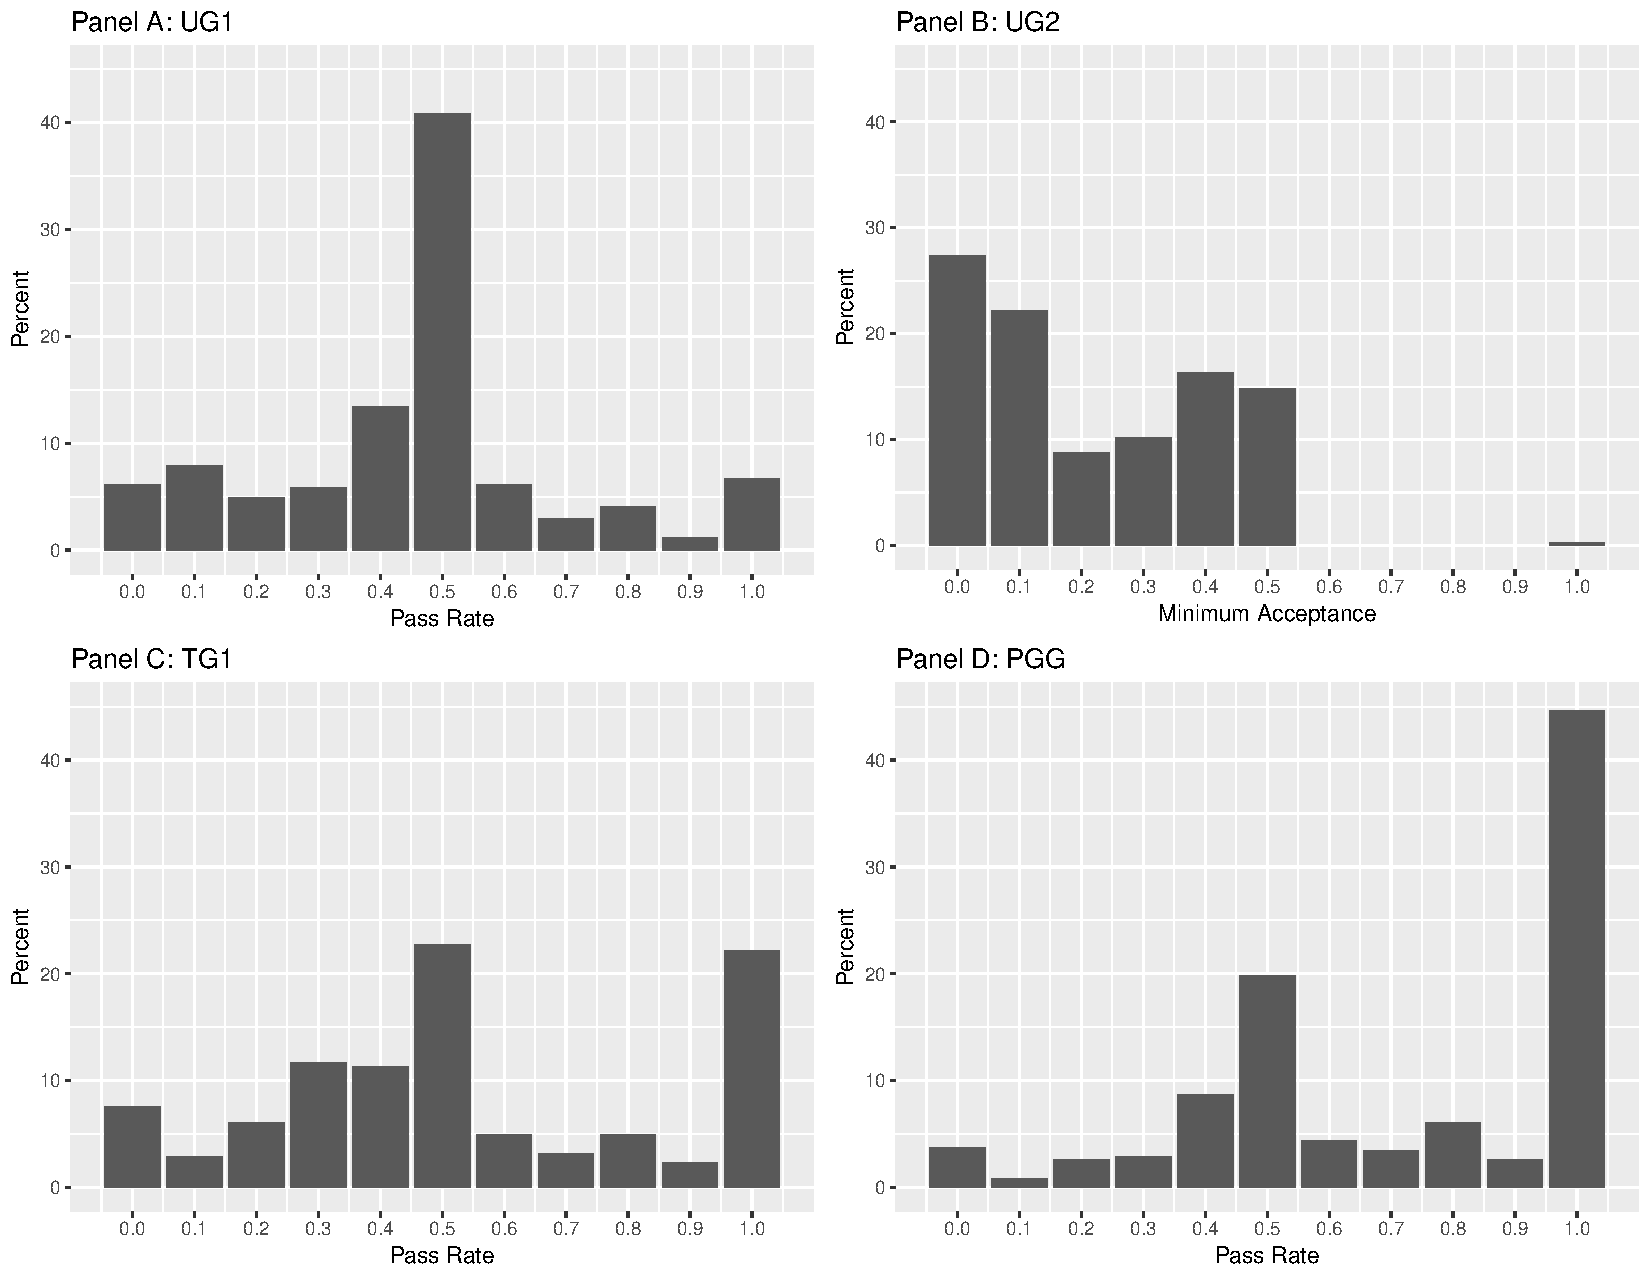
\includegraphics[scale=0.4]{Figure2a.pdf} \\



\noindent Figure 2: Distribution of responses in UG1, UG2, TG1, and PGG \\ \\
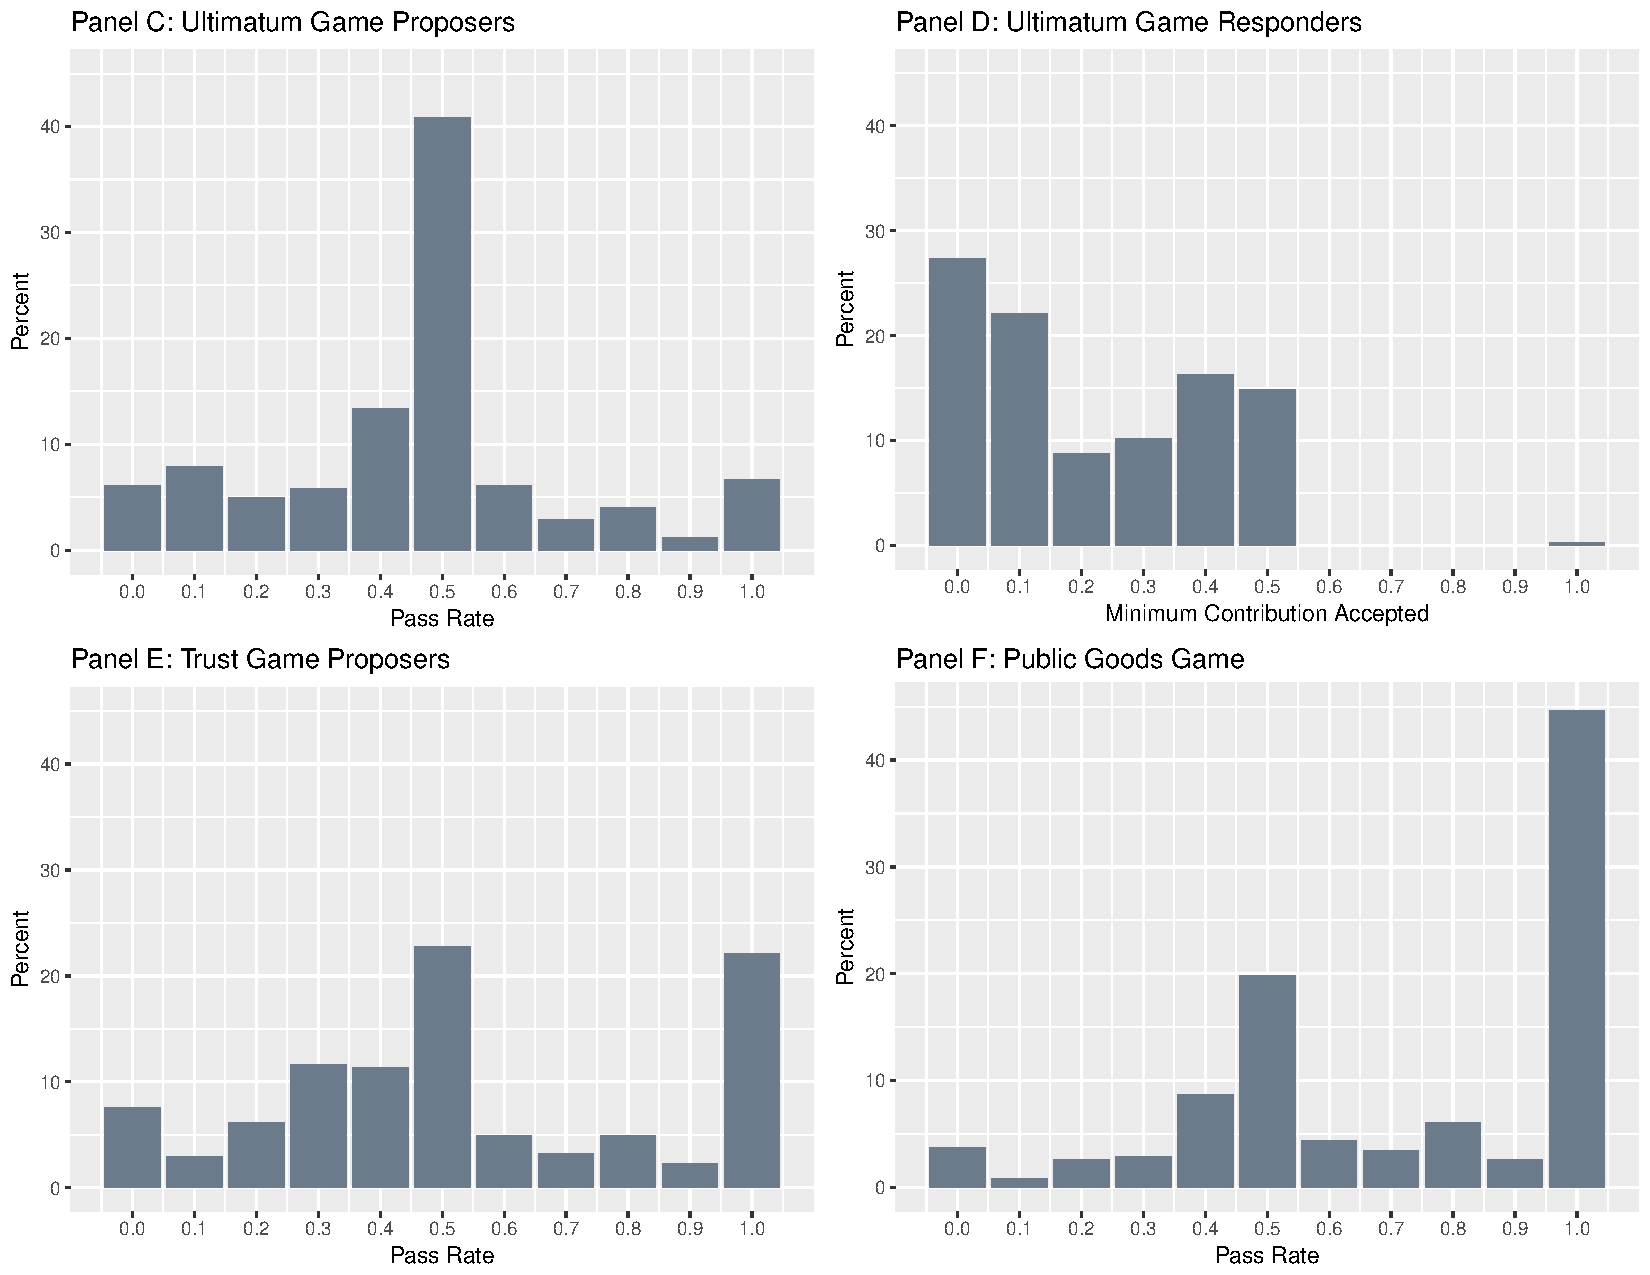
\includegraphics[scale=0.4]{Figure2b.pdf} \\

\noindent Figure 3: Distribution of responses from TG2 \\ \\
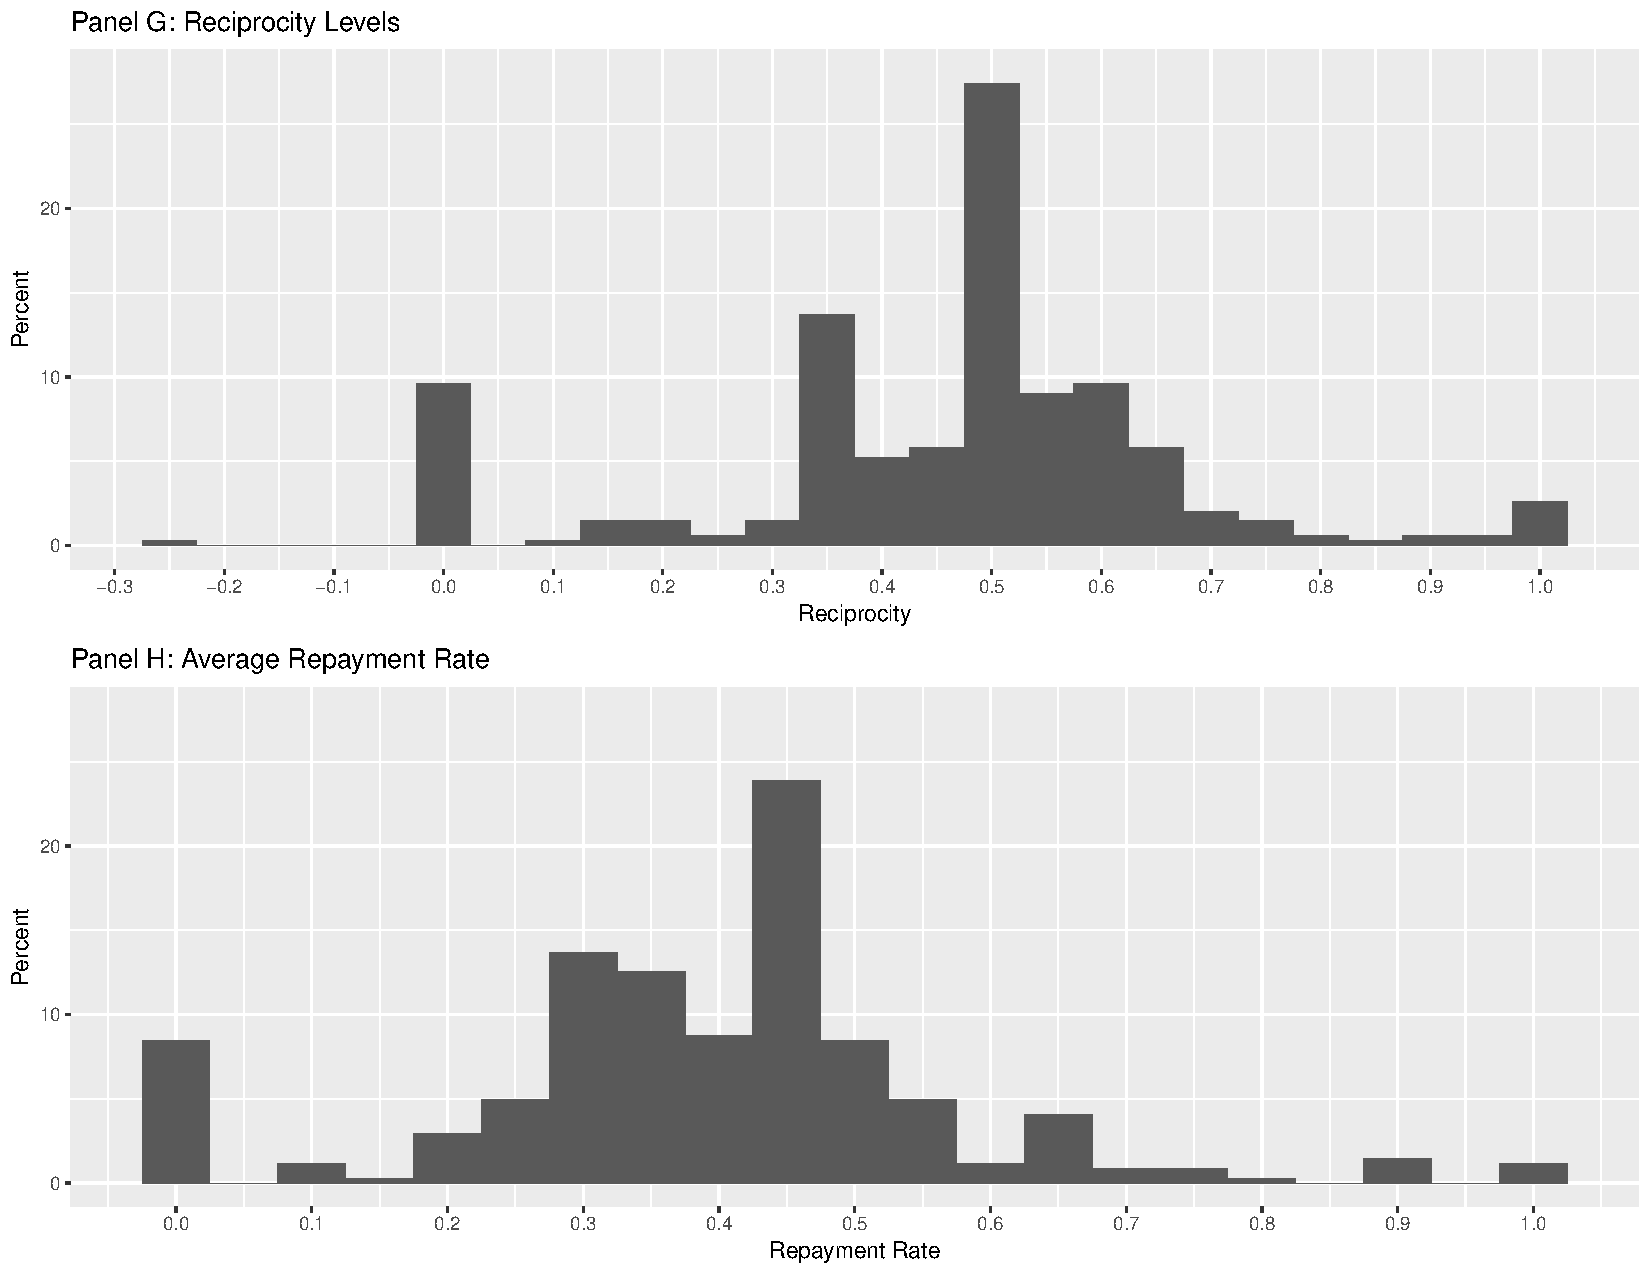
\includegraphics[scale=0.4]{Figure2c.pdf} \\



\noindent Figure 4: Total SRA scores\\ \\
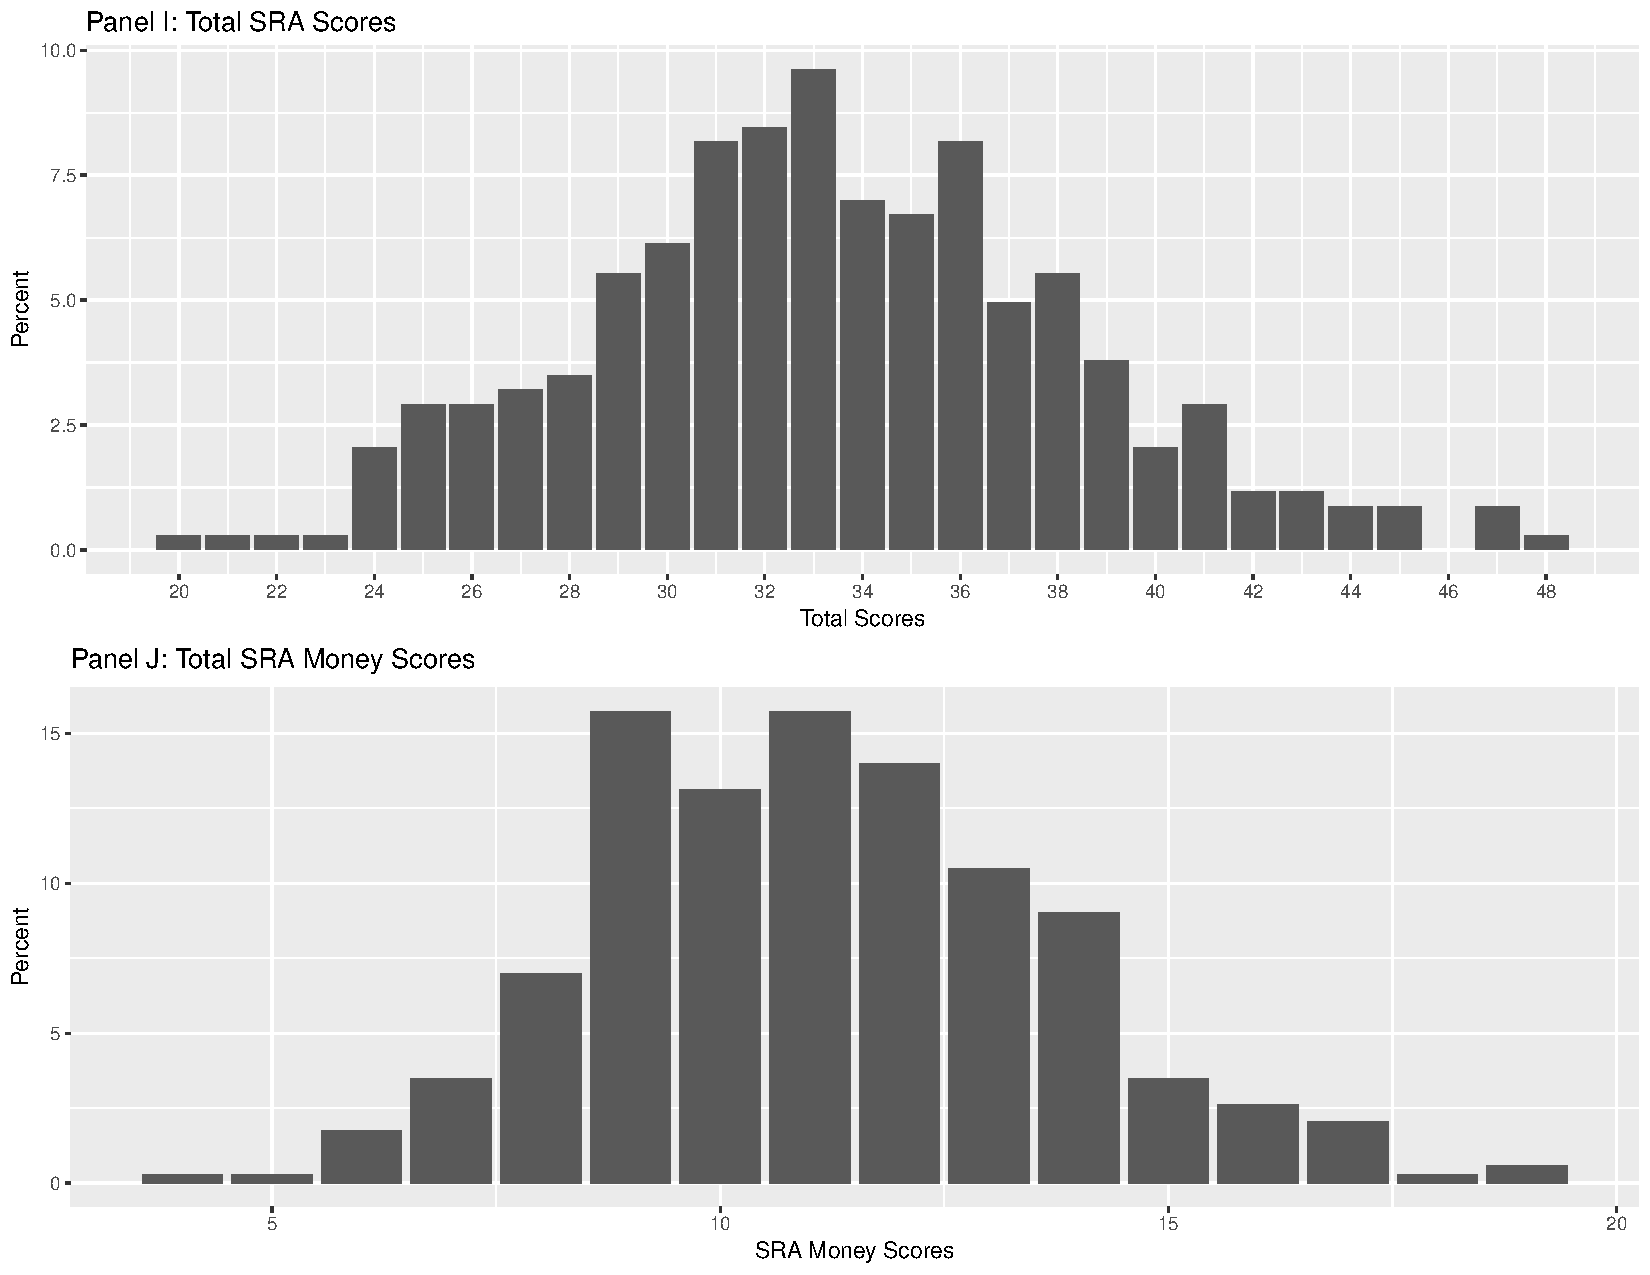
\includegraphics[scale=0.4]{Figure3.pdf}\\

\noindent Figure 5: Donations\\ \\
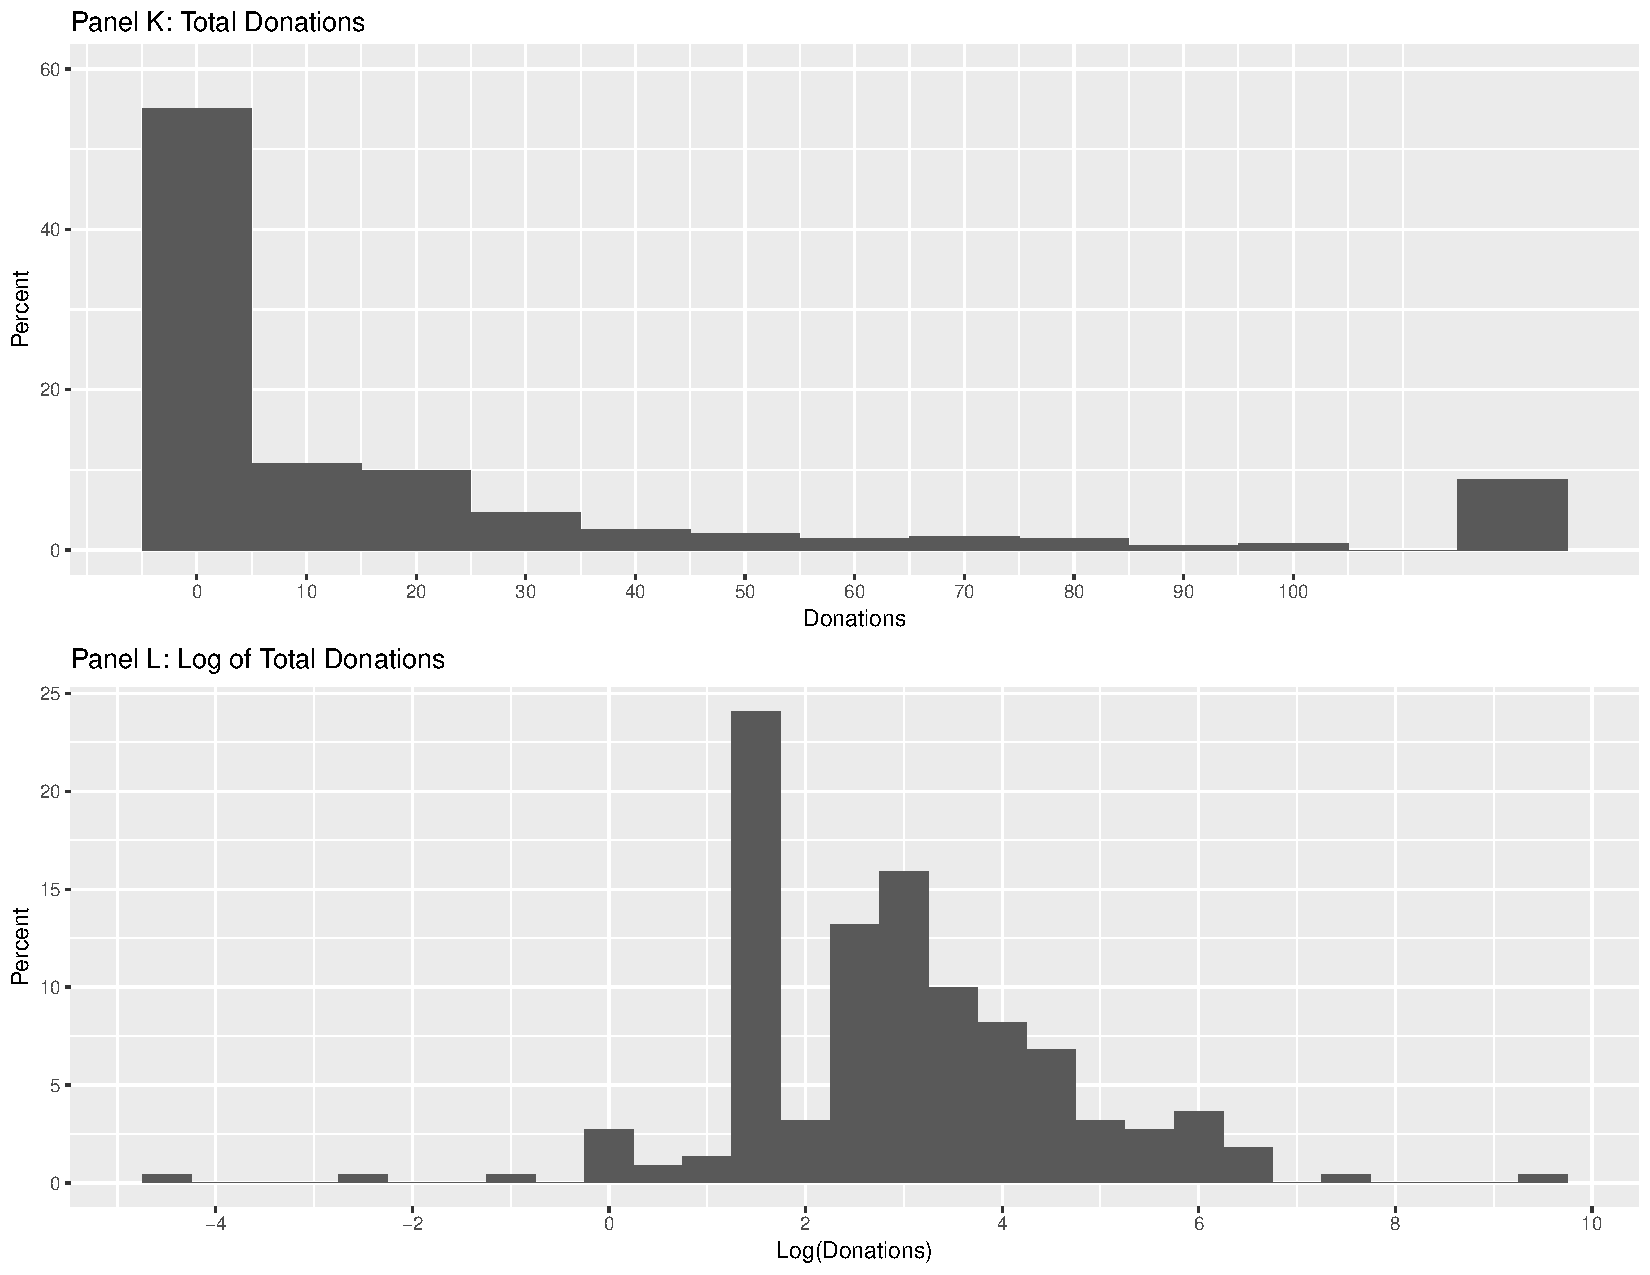
\includegraphics[scale=0.4]{Figure4.pdf}\\ \\



\begin{table}[!htbp] \centering 
  \caption{Pairwise correlations between game results (Spearman\rq s \(\rho\))} 
  \label{} \centering
  \begin{tabular}{rllllll}
  \hline
 & alpha &  \ UG1 & \ UG2 & \ TG1 & \ TG2 & \ PGG \\ 
  \hline
alpha &   \ 1.00  & -0.28*** & \ 0.04  & -0.26*** & -0.30*** & -0.16*** \\ 
  UG1 & -0.28*** & \ 1.00  &  \ 0.09  & \ 0.41*** & \ 0.31*** &  \ 0.30*** \\ 
  UG2 &  \ 0.04  &  \ 0.09  &  1.00  & -0.10* & -0.08  & -0.16*** \\ 
  TG1 & -0.26*** & \  0.41*** & -0.10* & \ 1.00  & \ 0.45*** &  \ 0.44*** \\ 
  TG2 & -0.30*** &  \ 0.31*** & -0.08  &  \ 0.45*** & \ 1.00  &  \ 0.21*** \\ 
  PGG & -0.16*** &  \ 0.30*** & -0.16*** & \  0.44*** & \ 0.21*** &  \ 1.00  \\ 
   \hline
      \textit{Note:}  & \multicolumn{6}{r}{$^{*}$p$<$0.1; $^{**}$p$<$0.05; $^{***}$p$<$0.01} \\ 
\end{tabular}
%\begin{tablenotes}\footnotesize
%\item Notes: 
%\item *, **,  and *** stand for statistical significance at the 10\%, 5\%, and 1\% levels.
%\item Alpha stands for \(\alpha\) levels derived from the generalized dictator game.
%\item UG1 and UG2 stand for Player 1 and Player 2 in ultimatum game, respectively.
%\item TG1 stands for Player 1 in trust game. 
%\item TG2 represents reciprocity levels for Player 2 in trust game.
%\item PGG stands for public goods game.
%\end{tablenotes}
\end{table}

\begin{table}[!htbp] \centering 
  \caption{Correlations between game results and SRA scores (Spearman\rq s \(\rho\))} 
  \label{} 
\centering
\begin{tabular}{rllllllll}
  \hline
 & SRAtotal & SRAmoney \\ 
  \hline
alpha  & -0.01  & \ \ -0.04  \\ 
  UG1  &  \ 0.02  &  \ \ \ 0.07  \\ 
  UG2 & -0.05  & \ \ -0.05  \\ 
  TG1 &  \ 0.07  &  \ \ \ 0.08  \\ 
  TG2  &  \ 0.04  & \ \ \  0.11** \\ 
  PGG  & \  0.06  &  \ \ \ 0.10* \\ 
  SRAtotal &  \ 1.00  &  \ \ \ 0.81*** \\ 
  SRAmoney  &  \ 0.81*** &  \ \ \ 1.00  \\ 
   \hline
   \textit{Note:}  & \multicolumn{2}{r}{$^{*}$p$<$0.1; $^{**}$p$<$0.05; $^{***}$p$<$0.01} \\ 
\end{tabular}
%\begin{tablenotes}\footnotesize
%\item Notes: 
%\item *, **,  and *** stand for statistical significance at the 10\%, 5\%, and 1\% levels.
%\item Alpha stands for \(\alpha\) levels derived from the generalized dictator game.
%\item UG1 and UG2 stand for Player 1 and Player 2 in ultimatum game, respectively.
%\item TG1 stands for Player 1 in trust game. 
%\item TG2 represents reciprocity levels for Player 2 in trust game.
%\item PGG stands for public goods game.
%\item SRAtotal stands for the total Self-Report Altruism score, and SRAmoney for those including only items related to money.
%\end{tablenotes}
\end{table}


\begin{table}[!htbp] \centering 
  \caption{Logistic regression models} 
  \label{} 
  \begin{adjustbox}{width=\textwidth}
\begin{tabular}{@{\extracolsep{5pt}}lcccccccccccc} 
\\[-1.8ex]\hline 
\hline \\[-1.8ex] 
 & \multicolumn{12}{c}{\textit{Dependent variable:}} \\ 
\cline{2-13} 
\\[-1.8ex] & \multicolumn{12}{c}{Donated} \\ 
\\[-1.8ex] & (1) & (2) & (3) & (4) & (5) & (6) & (7) & (8) & (9) & (10) & (11) & (12)\\ 
\hline \\[-1.8ex] 
 Alpha & 0.052 &  &  &  &  &  &  & 0.102 &  &  & 0.095 & 0.100 \\ 
  & (0.086) &  &  &  &  &  &  & (0.111) &  &  & (0.111) & (0.111) \\ 
  & & & & & & & & & & & & \\ 
 Rho &  & $-$0.00000 &  &  &  &  &  & $-$0.00001 &  &  & $-$0.00000 & $-$0.00001 \\ 
  &  & (0.00001) &  &  &  &  &  & (0.00001) &  &  & (0.00001) & (0.00001) \\ 
  & & & & & & & & & & & & \\ 
 UG1 &  &  & 0.016 &  &  &  &  & $-$0.003 &  &  & $-$0.001 & $-$0.008 \\ 
  &  &  & (0.107) &  &  &  &  & (0.125) &  &  & (0.125) & (0.125) \\ 
  & & & & & & & & & & & & \\ 
 UG2 &  &  &  & 0.120 &  &  &  & 0.125 &  &  & 0.132 & 0.133 \\ 
  &  &  &  & (0.137) &  &  &  & (0.142) &  &  & (0.142) & (0.142) \\ 
  & & & & & & & & & & & & \\ 
 TG1 &  &  &  &  & 0.011 &  &  & 0.019 &  &  & 0.011 & 0.020 \\ 
  &  &  &  &  & (0.083) &  &  & (0.108) &  &  & (0.108) & (0.108) \\ 
  & & & & & & & & & & & & \\ 
 Reciprocity &  &  &  &  &  & 0.025 &  & 0.046 &  &  & 0.043 & 0.030 \\ 
  &  &  &  &  &  & (0.120) &  & (0.140) &  &  & (0.140) & (0.140) \\ 
  & & & & & & & & & & & & \\ 
 PGG &  &  &  &  &  &  & 0.024 & 0.035 &  &  & 0.031 & 0.024 \\ 
  &  &  &  &  &  &  & (0.086) & (0.099) &  &  & (0.099) & (0.099) \\ 
  & & & & & & & & & & & & \\ 
 SRAtotal &  &  &  &  &  &  &  &  & 0.007 &  & 0.007 &  \\ 
  &  &  &  &  &  &  &  &  & (0.005) &  & (0.005) &  \\ 
  & & & & & & & & & & & & \\ 
 SRAmoney &  &  &  &  &  &  &  &  &  & 0.016 &  & 0.016 \\ 
  &  &  &  &  &  &  &  &  &  & (0.010) &  & (0.010) \\ 
  & & & & & & & & & & & & \\ 
 Constant & 0.614$^{***}$ & 0.640$^{***}$ & 0.634$^{***}$ & 0.616$^{***}$ & 0.635$^{***}$ & 0.630$^{***}$ & 0.624$^{***}$ & 0.499$^{***}$ & 0.400$^{**}$ & 0.461$^{***}$ & 0.270 & 0.333$^{**}$ \\ 
  & (0.052) & (0.028) & (0.056) & (0.039) & (0.052) & (0.061) & (0.067) & (0.127) & (0.176) & (0.117) & (0.212) & (0.165) \\ 
  & & & & & & & & & & & & \\ 
\hline \\[-1.8ex] 
Observations & 343 & 343 & 343 & 343 & 343 & 343 & 343 & 343 & 343 & 343 & 343 & 343 \\ 
Log Likelihood & $-$235.468 & $-$235.635 & $-$235.640 & $-$235.264 & $-$235.642 & $-$235.629 & $-$235.611 & $-$234.711 & $-$234.689 & $-$234.392 & $-$233.776 & $-$233.449 \\ 
Akaike Inf. Crit. & 474.937 & 475.270 & 475.280 & 474.528 & 475.284 & 475.258 & 475.222 & 485.423 & 473.378 & 472.785 & 485.551 & 484.898 \\ 
Psuedo-R$^{2}$ & 0.00078 & 0.000068 & 0.000048 & 0.00165 & 0.000039 & 0.000095 & 0.00017 & 0.00401 & 0.00410 & 0.00536 & 0.00799 & 0.00939 \\
\hline 
\hline \\[-1.8ex] 
\textit{Note:}  & \multicolumn{11}{r}{$^{*}$p$<$0.1; $^{**}$p$<$0.05; $^{***}$p$<$0.01} \\ 
\end{tabular} 
\end{adjustbox}
\end{table}


%\newpage
%
%\begin{table}[!htbp] \centering 
%  \caption{Tobit regression models} 
%  \label{} 
%            \begin{adjustbox}{width=\textwidth}
%\begin{tabular}{@{\extracolsep{5pt}}lcccccccccccc} 
%\\[-1.8ex]\hline 
%\hline \\[-1.8ex] 
% & \multicolumn{12}{c}{\textit{Dependent variable:}} \\ 
%\cline{2-13} 
%\\[-1.8ex] & \multicolumn{12}{c}{Donations} \\ 
%\\[-1.8ex] & (1) & (2) & (3) & (4) & (5) & (6) & (7) & (8) & (9) & (10) & (11) & (12) \\ 
%\hline \\[-1.8ex] 
% Alpha & 3.31909 &  &  &  &  &  &  & 9.490  &  & & 8.839 & 9.327 \\ 
%  & (6.74063) &  &  &  &  &  &  &  (8.557) & & & (8.519) & (8.469) \\ 
%  & & & & & & & & & & & & \\ 
% Rho &  & $-$0.00046 &  &  &  &  &   & $-$0.00084 & &  & $-$0.000767 & $-$0.000812 \\ 
%  &  & (0.00058) &  &  &  &  &  & (0.000696) &  &  & (0.000694) & (0.000690) \\ 
%  & & & & & & & & & & & & \\  
% UG1 &  & & 6.86161 &  &  &  &  & 6.963 &  &  & 7.380 & 6.553 \\ 
%  &  & & (8.35099) &  &  &  &  & (9.479) &  &  & (9.443) & (9.394) \\ 
%  & & & & & & & & & & & & \\ 
% UG2 &  &  & & 6.02451 &  &  &  & 5.842 &  &  & 6.479 & 6.674 \\ 
%  &  &  & & (10.74423) &  &  &  & (1.093) &  &  & (10.89) & (10.84) \\ 
%  & & & & & & & & & & & & \\ 
% TG1 &  &  &  & & 0.40224 &  &  & $-$0.2433 &  &  & $-$1.226 & $-$0.2985 \\ 
%  &  &  &  & & (6.48083) &  &   & (8.273)  &  &  & (8.260) & (8.197) \\ 
%  & & & & & & & & & & & &\\ 
% TG2 &  &  &  &  & & $-$7.78095 &   & $-$10.01 &  &  & $-$10.27 & $-$11.95 \\ 
%  &  &  &  &  & & (9.33936) &   & (10.67) &  &  & (10.62) & (10.60) \\ 
%  & & & & & & & & & & & &\\ 
% PGG &  &  &  &  &  & & 9.74202  & 11.13 &  &  & 10.89 & 9.913 \\ 
%  &  &  &  &  &  & & (6.73445)  & (7.594) &  &  & (7.566) & (7.542) \\ 
%  & & & & & & & & & & & &\\ 
% SRAtotal &  &  &  &  &  &  & & & 0.70389$^{*}$ &  & 0.6842$^{*}$ &  \\ 
%  &  &  &  &  &  &  & & & (0.40552) &  & (0.4033) &  \\ 
%  & & & & & & & & & & & \\ 
% SRAmoney &  &  &  &  &  &  &  & & & 1.95175$^{**}$ &  & 1.943$^{**}$ \\ 
%  &  &  &  &  &  &  &  & & & (0.79090) &  & (0.7893) \\ 
%  & & & & & & & & & & & &\\ 
% Constant & 7.12277$^{*}$ & 8.21167$^{***}$ & 5.71272 & 7.56796$^{**}$ & 8.63908$^{**}$ & 12.43205$^{***}$ & 1.89668 & $-$4.951 & $-$14.61146 & $-$12.89298 & $-$26.82 & $-$24.68$^{*}$ \\ 
%  & (4.10025) & (2.22776) & (4.37273) & (3.10718) & (4.09095) & (4.73771) & (5.27791) & (9.886) & (13.73187) & (9.12441) & (16.31) & (12.75) \\ 
%  & & & & & & & & & & & \\ 
%\hline \\[-1.8ex] 
%Observations & 343 & 343 & 343 & 343 & 343 & 343 & 343 & 343 & 343 & 343 & 343 & 343 \\ 
%Pseudo-R$^{2}$ & 0.000124 & 0.000325 & 0.000346 & 0.000161 & 0.000002 & 0.000356 & 0.001073 & 0.0031697 & 0.001548 & 0.003140 & 0.004650 & 0.006297\\
%\hline 
%\hline \\[-1.8ex] 
%\textit{Note:}  & \multicolumn{11}{r}{$^{*}$p$<$0.1; $^{**}$p$<$0.05; $^{***}$p$<$0.01} \\ 
%\end{tabular} 
%\end{adjustbox}
%\end{table} 

\begin{table}[!htbp] \centering 
  \caption{Linear regression models} 
  \label{} 
   \begin{adjustbox}{width=\textwidth}
\begin{tabular}{@{\extracolsep{5pt}}lcccccccccccc} 
\\[-1.8ex]\hline 
\hline \\[-1.8ex] 
 & \multicolumn{12}{c}{\textit{Dependent variable:}} \\ 
\cline{2-13} 
\\[-1.8ex] & \multicolumn{12}{c}{Log(Donations)} \\ 
\\[-1.8ex] & (1) & (2) & (3) & (4) & (5) & (6) & (7) & (8) & (9) & (10) & (11) & (12)\\ 
\hline \\[-1.8ex] 
 Alpha & 0.080 &  &  &  &  &  &  & 0.414 &  &  & 0.403 & 0.429 \\ 
  & (0.383) &  &  &  &  &  &  & (0.492) &  &  & (0.493) & (0.491) \\ 
  & & & & & & & & & & & & \\ 
 Rho &  & $-$0.00003 &  &  &  &  &  & $-$0.0001 &  &  & $-$0.00005 & $-$0.0001 \\ 
  &  & (0.00003) &  &  &  &  &  & (0.00004) &  &  & (0.00004) & (0.00004) \\ 
  & & & & & & & & & & & & \\ 
 UG1 &  &  & 0.488 &  &  &  &  & 0.707 &  &  & 0.725 & 0.695 \\ 
  &  &  & (0.454) &  &  &  &  & (0.506) &  &  & (0.506) & (0.504) \\ 
  & & & & & & & & & & & & \\ 
 UG2 &  &  &  & $-$0.270 &  &  &  & $-$0.350 &  &  & $-$0.325 & $-$0.322 \\ 
  &  &  &  & (0.590) &  &  &  & (0.598) &  &  & (0.599) & (0.597) \\ 
  & & & & & & & & & & & & \\ 
 TG1 &  &  &  &  & $-$0.210 &  &  & $-$0.325 &  &  & $-$0.358 & $-$0.320 \\ 
  &  &  &  &  & (0.365) &  &  & (0.464) &  &  & (0.466) & (0.463) \\ 
  & & & & & & & & & & & & \\ 
 Reciprocity &  &  &  &  &  & $-$0.713 &  & $-$0.787 &  &  & $-$0.799 & $-$0.851 \\ 
  &  &  &  &  &  & (0.516) &  & (0.600) &  &  & (0.600) & (0.600) \\ 
  & & & & & & & & & & & & \\ 
 PGG &  &  &  &  &  &  & 0.635$^{*}$ & 0.685 &  &  & 0.691 & 0.652 \\ 
  &  &  &  &  &  &  & (0.383) & (0.421) &  &  & (0.422) & (0.421) \\ 
  & & & & & & & & & & & & \\ 
 SRAtotal &  &  &  &  &  &  &  &  & 0.017 &  & 0.018 &  \\ 
  &  &  &  &  &  &  &  &  & (0.022) &  & (0.023) &  \\ 
  & & & & & & & & & & & & \\ 
 SRAmoney &  &  &  &  &  &  &  &  &  & 0.064 &  & 0.064 \\ 
  &  &  &  &  &  &  &  &  &  & (0.043) &  & (0.043) \\ 
  & & & & & & & & & & & & \\ 
 Constant & 2.903$^{***}$ & 2.896$^{***}$ & 2.721$^{***}$ & 3.005$^{***}$ & 3.060$^{***}$ & 3.272$^{***}$ & 2.487$^{***}$ & 2.447$^{***}$ & 2.377$^{***}$ & 2.221$^{***}$ & 1.839$^{**}$ & 1.768$^{**}$ \\ 
  & (0.232) & (0.121) & (0.238) & (0.171) & (0.229) & (0.262) & (0.298) & (0.565) & (0.763) & (0.502) & (0.932) & (0.729) \\ 
  & & & & & & & & & & & & \\ 
\hline \\[-1.8ex] 
Observations & 220 & 220 & 220 & 220 & 220 & 220 & 220 & 220 & 220 & 220 & 220 & 220 \\ 
R$^{2}$ & 0.0002 & 0.005 & 0.005 & 0.001 & 0.002 & 0.009 & 0.012 & 0.043 & 0.003 & 0.010 & 0.046 & 0.053 \\ 
Adjusted R$^{2}$ & $-$0.004 & 0.001 & 0.001 & $-$0.004 & $-$0.003 & 0.004 & 0.008 & 0.011 & $-$0.002 & 0.005 & 0.010 & 0.017 \\ 
Residual Std. Error & 1.668 & 1.663 & 1.663 & 1.667 & 1.667 & 1.661 & 1.657 & 1.654 & 1.666  & 1.660 & 1.656  & 1.650 \\ 
& (df = 218) & (df = 218) & (df = 218) & (df = 218) & (df = 218) & (df = 218) & (df = 218) & (df = 218) & (df = 218) & (df = 218) & (df = 218) & (df = 218) \\
F Statistic & 0.044 & 1.149  & 1.155 & 0.210  & 0.331 & 1.907 & 2.749$^{*}$ & 1.363 & 0.568 & 2.190 & 1.275  & 1.469 \\ 
& (df = 1; 218) & (df = 1; 218) & (df = 1; 218) & (df = 1; 218) & (df = 1; 218) & (df = 1; 218) & (df = 1; 218) & (df = 1; 218) & (df = 1; 218) & (df = 1; 218) & (df = 1; 218) & (df = 1; 218) \\
\hline 
\hline \\[-1.8ex] 
\textit{Note:}  & \multicolumn{12}{r}{$^{*}$p$<$0.1; $^{**}$p$<$0.05; $^{***}$p$<$0.01} \\ 
\end{tabular} 
\end{adjustbox}
\end{table} 






\begin{table}[!htbp] \centering 
  \caption{Best-subset logistic regression} 
  \label{} 
\begin{tabular}{@{\extracolsep{5pt}}lc} 
\\[-1.8ex]\hline 
\hline \\[-1.8ex] 
 & \multicolumn{1}{c}{\textit{Dependent variable:}} \\ 
\cline{2-2} 
\\[-1.8ex] & Donated \\ 
\hline \\[-1.8ex] 
 SRA3 & $-$0.096$^{***}$ \\ 
  & (0.028) \\ 
  & \\ 
 SRA4 & 0.123$^{***}$ \\ 
  & (0.030) \\ 
  & \\ 
 SRA8 & 0.075$^{**}$ \\ 
  & (0.034) \\ 
  & \\ 
 SRA10 & $-$0.052$^{**}$ \\ 
  & (0.025) \\ 
  & \\ 
 Constant & 0.386$^{**}$ \\ 
  & (0.155) \\ 
  & \\ 
\hline \\[-1.8ex] 
Observations & 343 \\ 
Log Likelihood & $-$220.385 \\ 
Akaike Inf. Crit. & 450.770 \\ 
Psuedo-R$^{2}$ & 0.06506 \\
\hline 
\hline \\[-1.8ex] 
\textit{Note:}  & \multicolumn{1}{r}{$^{*}$p$<$0.1; $^{**}$p$<$0.05; $^{***}$p$<$0.01} \\ 
\end{tabular} 
\end{table} 


%\begin{table}[!htbp] \centering 
%  \caption{Best-subset tobit regression} 
%  \label{} 
%\begin{tabular}{@{\extracolsep{5pt}}lc} 
%\\[-1.8ex]\hline 
%\hline \\[-1.8ex] 
% & \multicolumn{1}{c}{\textit{Dependent variable:}} \\ 
%\cline{2-2} 
%\\[-1.8ex] & Donations \\ 
%\hline \\[-1.8ex] 
% Rho & $-$0.0004592 \\ 
%  & (0.0005748) \\ 
%  & \\ 
% Constant & 8.21167$^{***}$ \\ 
%  & (2.22776) \\ 
%  & \\ 
%\hline \\[-1.8ex] 
%Observations & 343 \\ 
%Psuedo-R$^{2}$ & 0.000325 \\
%\hline 
%\hline \\[-1.8ex] 
%\textit{Note:}  & \multicolumn{1}{r}{$^{*}$p$<$0.1; $^{**}$p$<$0.05; $^{***}$p$<$0.01} \\ 
%\end{tabular} 
%\end{table} 

\begin{table}[!htbp] \centering 
  \caption{Best-subset linear regresion} 
  \label{} 
\begin{tabular}{@{\extracolsep{5pt}}lc} 
\\[-1.8ex]\hline 
\hline \\[-1.8ex] 
 & \multicolumn{1}{c}{\textit{Dependent variable:}} \\ 
\cline{2-2} 
\\[-1.8ex] & Log(Donations) \\ 
\hline \\[-1.8ex] 
 UG1 & 0.960$^{**}$ \\ 
  & (0.446) \\ 
  & \\ 
 TG2 & $-$1.387$^{***}$ \\ 
  & (0.511) \\ 
  & \\ 
 SRA3 & $-$0.220$^{*}$ \\ 
  & (0.122) \\ 
  & \\ 
 SRA4 & 0.744$^{***}$ \\ 
  & (0.142) \\ 
  & \\ 
 SRA5 & $-$0.414$^{***}$ \\ 
  & (0.131) \\ 
  & \\ 
 SRA6 & 0.254$^{*}$ \\ 
  & (0.147) \\ 
  & \\ 
 Constant & 1.592$^{*}$ \\ 
  & (0.838) \\ 
  & \\ 
\hline \\[-1.8ex] 
Observations & 220 \\ 
R$^{2}$ & 0.157 \\ 
Adjusted R$^{2}$ & 0.133 \\ 
Residual Std. Error & 1.549 (df = 213) \\ 
F Statistic & 6.604$^{***}$ (df = 6; 213) \\ 
\hline 
\hline \\[-1.8ex] 
\textit{Note:}  & \multicolumn{1}{r}{$^{*}$p$<$0.1; $^{**}$p$<$0.05; $^{***}$p$<$0.01} \\ 
\end{tabular} 
\end{table} 


\begin{table}[!htbp] \centering 
  \caption{Logistic predictive models} 
  \label{} 
     \begin{adjustbox}{width=\textwidth}
\begin{tabular}{@{\extracolsep{5pt}}lcccccccccccc} 
\\[-1.8ex]\hline 
\hline \\[-1.8ex] 
 & \multicolumn{12}{c}{\textit{Dependent variable:}} \\ 
\cline{2-13} 
\\[-1.8ex] & \multicolumn{12}{c}{Donated} \\ 
\\[-1.8ex] & (1) & (2) & (3) & (4) & (5) & (6) & (7) & (8) & (9) & (10) & (11) & (12)\\ 
\hline \\[-1.8ex] 
 Alpha & 0.109 &  &  &  &  &  &  & 0.122 &  &  & 0.125 & 0.130 \\ 
  & (0.088) &  &  &  &  &  &  & (0.115) &  &  & (0.115) & (0.115) \\ 
  & & & & & & & & & & & & \\ 
 Rho &  & 0.00000 &  &  &  &  &  & $-$0.00000 &  &  & 0.00000 & $-$0.00000 \\ 
  &  & (0.00001) &  &  &  &  &  & (0.00001) &  &  & (0.00001) & (0.00001) \\ 
  & & & & & & & & & & & & \\ 
 Ultimatum1 &  &  & $-$0.041 &  &  &  &  & $-$0.064 &  &  & $-$0.057 & $-$0.064 \\ 
  &  &  & (0.110) &  &  &  &  & (0.128) &  &  & (0.128) & (0.127) \\ 
  & & & & & & & & & & & & \\ 
 Ultimatum2 &  &  &  & 0.242$^{*}$ &  &  &  & 0.248$^{*}$ &  &  & 0.256$^{*}$ & 0.259$^{*}$ \\ 
  &  &  &  & (0.141) &  &  &  & (0.145) &  &  & (0.145) & (0.145) \\ 
  & & & & & & & & & & & & \\ 
 Trust1 &  &  &  &  & 0.003 &  &  & 0.021 &  &  & 0.012 & 0.023 \\ 
  &  &  &  &  & (0.087) &  &  & (0.109) &  &  & (0.109) & (0.109) \\ 
  & & & & & & & & & & & & \\ 
 Trust2 &  &  &  &  &  & 0.075 &  & 0.157 &  &  & 0.166 & 0.153 \\ 
  &  &  &  &  &  & (0.124) &  & (0.143) &  &  & (0.143) & (0.143) \\ 
  & & & & & & & & & & & & \\ 
 Cooperation &  &  &  &  &  &  & $-$0.030 & $-$0.009 &  &  & $-$0.016 & $-$0.023 \\ 
  &  &  &  &  &  &  & (0.091) & (0.104) &  &  & (0.104) & (0.104) \\ 
  & & & & & & & & & & & & \\ 
 SRAtotal &  &  &  &  &  &  &  &  & 0.005 &  & 0.006 &  \\ 
  &  &  &  &  &  &  &  &  & (0.005) &  & (0.005) &  \\ 
  & & & & & & & & & & & & \\ 
 SRAmoney &  &  &  &  &  &  &  &  &  & 0.013 &  & 0.015 \\ 
  &  &  &  &  &  &  &  &  &  & (0.011) &  & (0.011) \\ 
  & & & & & & & & & & & & \\ 
 Constant & 0.677$^{***}$ & 0.740$^{***}$ & 0.752$^{***}$ & 0.680$^{***}$ & 0.731$^{***}$ & 0.698$^{***}$ & 0.755$^{***}$ & 0.570$^{***}$ & 0.559$^{***}$ & 0.588$^{***}$ & 0.358 & 0.405$^{**}$ \\ 
  & (0.052) & (0.029) & (0.059) & (0.041) & (0.055) & (0.063) & (0.072) & (0.132) & (0.183) & (0.123) & (0.227) & (0.177) \\ 
  & & & & & & & & & & & & \\ 
\hline \\[-1.8ex] 
Observations & 273 & 273 & 273 & 273 & 273 & 273 & 273 & 273 & 273 & 273 & 273 & 273 \\ 
Log Likelihood & $-$165.074 & $-$165.629 & $-$165.784 & $-$164.378 & $-$165.852 & $-$165.669 & $-$165.797 & $-$162.950 & $-$165.393 & $-$165.126 & $-$162.267 & $-$161.945 \\ 
Akaike Inf. Crit. & 334.148 & 335.258 & 335.568 & 332.756 & 335.703 & 335.339 & 335.594 & 341.899 & 334.785 & 334.251 & 342.534 & 341.890 \\ 
MSPE & 0.40956 & 0.40779 & 0.40543 & 0.41134 & 0.40374 & 0.40520 & 0.40555 & 0.42300 & 0.39969 & 0.39818 & 0.42041 & 0.41904 \\
\hline 
\hline \\[-1.8ex] 
\textit{Note:}  & \multicolumn{12}{r}{$^{*}$p$<$0.1; $^{**}$p$<$0.05; $^{***}$p$<$0.01} \\ 
\end{tabular} 
\end{adjustbox}
\end{table} 


\begin{table}[!htbp] \centering 
  \caption{Best subsets logistic predictive models} 
  \label{} 
  \begin{adjustbox}{width=\textwidth}
\begin{tabular}{@{\extracolsep{5pt}}lccccc} 
\\[-1.8ex]\hline 
\hline \\[-1.8ex] 
 & \multicolumn{5}{c}{\textit{Dependent variable:}} \\ 
\cline{2-6} 
\\[-1.8ex] & \multicolumn{5}{c}{Donated} \\ 
\\[-1.8ex] & (1) & (2) & (3) & (4) & (5)\\ 
\hline \\[-1.8ex] 
 Alpha & 0.164$^{*}$ & 0.137 &  & 0.149$^{*}$ & 0.146$^{*}$ \\ 
  & (0.088) & (0.085) &  & (0.085) & (0.085) \\ 
  & & & & & \\ 
 Ultimatum2 & 0.201 & 0.184 & 0.202 &  &  \\ 
  & (0.138) & (0.138) & (0.138) &  &  \\ 
  & & & & & \\ 
 Avg Return & 0.176 &  &  &  &  \\ 
  & (0.146) &  &  &  &  \\ 
  & & & & & \\ 
 SRA3 & $-$0.075$^{**}$ & $-$0.079$^{***}$ & $-$0.076$^{**}$ & $-$0.083$^{***}$ & $-$0.084$^{***}$ \\ 
  & (0.030) & (0.029) & (0.029) & (0.029) & (0.029) \\ 
  & & & & & \\ 
 SRA4 & 0.126$^{***}$ & 0.127$^{***}$ & 0.123$^{***}$ & 0.132$^{***}$ & 0.128$^{***}$ \\ 
  & (0.030) & (0.030) & (0.030) & (0.030) & (0.030) \\ 
  & & & & & \\ 
 SR10 &  &  &  & $-$0.026 &  \\ 
  &  &  &  & (0.024) &  \\ 
  & & & & & \\ 
 Constant & 0.342$^{**}$ & 0.436$^{***}$ & 0.508$^{***}$ & 0.547$^{***}$ & 0.484$^{***}$ \\ 
  & (0.155) & (0.134) & (0.127) & (0.142) & (0.129) \\ 
  & & & & & \\ 
\hline \\[-1.8ex] 
Observations & 273 & 273 & 273 & 273 & 273 \\ 
Log Likelihood & $-$152.803 & $-$153.545 & $-$154.861 & $-$153.852 & $-$154.452 \\ 
Akaike Inf. Crit. & 317.605 & 317.091 & 317.722 & 317.704 & 316.904 \\ 
MSPE & 0.39857 & 0.39310 & 0.38511 & 0.38435 & 0.38955 \\
\hline 
\hline \\[-1.8ex] 
\textit{Note:}  & \multicolumn{5}{r}{$^{*}$p$<$0.1; $^{**}$p$<$0.05; $^{***}$p$<$0.01} \\ 
\end{tabular} 
\end{adjustbox}
\end{table} 

\begin{table}[!htbp] \centering 
  \caption{Lasso penalized logistic predictive model} 
  \label{} 
\begin{tabular}{@{\extracolsep{5pt}}lc} 
\\[-1.8ex]\hline 
\hline \\[-1.8ex] 
 & \multicolumn{1}{c}{\textit{Dependent variable:}} \\ 
\cline{2-2} 
\\[-1.8ex] & Donated \\ 
\hline \\[-1.8ex] 
 Alpha & 0.038536 \\ 
  & \\ 
 Ultimatum2 & 0.071665 \\ 
  & \\ 
 SRA3 & $-$0.040027 \\ 
  & \\ 
 SRA4 & 0.083644$^{***}$ \\ 
  & \\ 
 Constant & 0.538420 \\ 
  & \\ 
\hline \\[-1.8ex] 
Observations & 343 \\ 
MSPE & 0.39048 \\
\hline 
\hline \\[-1.8ex] 
\textit{Note:}  & \multicolumn{1}{r}{$^{*}$p$<$0.1; $^{**}$p$<$0.05; $^{***}$p$<$0.01} \\ 
\end{tabular} 
\end{table} 


\begin{table}[!htbp] \centering 
  \caption{Linear predictive models} 
  \label{} 
  \begin{adjustbox}{width=\textwidth}
\begin{tabular}{@{\extracolsep{5pt}}lcccccccccccc} 
\\[-1.8ex]\hline 
\hline \\[-1.8ex] 
 & \multicolumn{12}{c}{\textit{Dependent variable:}} \\ 
\cline{2-13} 
\\[-1.8ex] & \multicolumn{12}{c}{Log(Donations)} \\ 
\\[-1.8ex] & (1) & (2) & (3) & (4) & (5) & (6) & (7) & (8) & (9) & (10) & (11) & (12)\\ 
\hline \\[-1.8ex] 
 Alpha & 0.002 &  &  &  &  &  &  & 0.462 &  &  & 0.469 & 0.504 \\ 
  & (0.397) &  &  &  &  &  &  & (0.508) &  &  & (0.508) & (0.507) \\ 
  & & & & & & & & & & & & \\ 
 Rho &  & $-$0.00005 &  &  &  &  &  & $-$0.0001 &  &  & $-$0.0001 & $-$0.0001 \\ 
  &  & (0.00003) &  &  &  &  &  & (0.00004) &  &  & (0.00004) & (0.00004) \\ 
  & & & & & & & & & & & & \\ 
 Ultimatum1 &  &  & 0.480 &  &  &  &  & 0.664 &  &  & 0.704 & 0.670 \\ 
  &  &  & (0.482) &  &  &  &  & (0.535) &  &  & (0.536) & (0.533) \\ 
  & & & & & & & & & & & & \\ 
 Ultimatum2 &  &  &  & $-$0.233 &  &  &  & $-$0.346 &  &  & $-$0.296 & $-$0.276 \\ 
  &  &  &  & (0.616) &  &  &  & (0.625) &  &  & (0.627) & (0.624) \\ 
  & & & & & & & & & & & & \\ 
 Trust1 &  &  &  &  & $-$0.234 &  &  & $-$0.311 &  &  & $-$0.360 & $-$0.312 \\ 
  &  &  &  &  & (0.389) &  &  & (0.484) &  &  & (0.487) & (0.483) \\ 
  & & & & & & & & & & & & \\ 
 Trust2 &  &  &  &  &  & $-$0.624 &  & $-$0.713 &  &  & $-$0.698 & $-$0.739 \\ 
  &  &  &  &  &  & (0.551) &  & (0.631) &  &  & (0.631) & (0.629) \\ 
  & & & & & & & & & & & & \\ 
 Cooperation &  &  &  &  &  &  & 0.507 & 0.579 &  &  & 0.586 & 0.538 \\ 
  &  &  &  &  &  &  & (0.408) & (0.447) &  &  & (0.447) & (0.446) \\ 
  & & & & & & & & & & & & \\ 
 SRAtotal &  &  &  &  &  &  &  &  & 0.024 &  & 0.025 &  \\ 
  &  &  &  &  &  &  &  &  & (0.024) &  & (0.024) &  \\ 
  & & & & & & & & & & & & \\ 
 SRAmoney &  &  &  &  &  &  &  &  &  & 0.074 &  & 0.073 \\ 
  &  &  &  &  &  &  &  &  &  & (0.046) &  & (0.047) \\ 
  & & & & & & & & & & & & \\ 
 Constant & 2.999$^{***}$ & 2.930$^{***}$ & 2.775$^{***}$ & 3.053$^{***}$ & 3.129$^{***}$ & 3.288$^{***}$ & 2.631$^{***}$ & 2.508$^{***}$ & 2.193$^{***}$ & 2.156$^{***}$ & 1.666 & 1.673$^{**}$ \\ 
  & (0.239) & (0.127) & (0.255) & (0.183) & (0.245) & (0.280) & (0.320) & (0.596) & (0.817) & (0.541) & (1.024) & (0.797) \\ 
  & & & & & & & & & & & & \\ 
\hline \\[-1.8ex] 
Observations & 200 & 200 & 200 & 200 & 200 & 200 & 200 & 200 & 200 & 200 & 200 & 200 \\ 
R$^{2}$ & 0.00000 & 0.010 & 0.005 & 0.001 & 0.002 & 0.006 & 0.008 & 0.041 & 0.005 & 0.013 & 0.046 & 0.053 \\ 
Adjusted R$^{2}$ & $-$0.005 & 0.005 & $-$0.00003 & $-$0.004 & $-$0.003 & 0.001 & 0.003 & 0.006 & $-$0.00002 & 0.008 & 0.006 & 0.014 \\ 
Residual Std. Error & 1.668 & 1.660  & 1.664 & 1.668 & 1.667  & 1.663 & 1.662  & 1.659  & 1.664  & 1.658 & 1.659  & 1.653  \\ 
& (df = 198) & (df = 198) & (df = 198) & (df = 198) & (df = 198) & (df = 198) & (df = 198) & (df = 198) & (df = 198) & (df = 198) & (df = 198) & (df = 198) \\
F Statistic & 0.00003 & 2.100  & 0.994  & 0.143 & 0.362  & 1.283 & 1.540  & 1.175 & 0.996 & 2.555 & 1.156  & 1.345  \\ 
& (df = 1; 198) & (df = 1; 198) & (df = 1; 198) & (df = 1; 198) & (df = 1; 198) & (df = 1; 198) & (df = 1; 198) & (df = 1; 198) & (df = 1; 198) & (df = 1; 198) & (df = 1; 198) & (df = 1; 198)  \\
MSPE & 7.57299 & 7.46333 & 7.45320 & 7.60122 & 7.61780 & 7.60167 & 7.42111 & 7.34503 & 7.44099 & 7.26722 & 7.21150 & 7.05559 \\
\hline 
\hline \\[-1.8ex] 
\textit{Note:}  & \multicolumn{12}{r}{$^{*}$p$<$0.1; $^{**}$p$<$0.05; $^{***}$p$<$0.01} \\ 
\end{tabular} 
\end{adjustbox}
\end{table}


\begin{table}[!htbp] \centering 
  \caption{Best subset linear predictive models} 
  \label{} 
    \begin{adjustbox}{width=\textwidth}
\begin{tabular}{@{\extracolsep{5pt}}lccccc} 
\\[-1.8ex]\hline 
\hline \\[-1.8ex] 
 & \multicolumn{5}{c}{\textit{Dependent variable:}} \\ 
\cline{2-6} 
\\[-1.8ex] & \multicolumn{5}{c}{Log(Donations)} \\ 
\\[-1.8ex] & (1) & (2) & (3) & (4) & (5)\\ 
\hline \\[-1.8ex] 
 Rho & $-$0.00004 &  &  &  &  \\ 
  & (0.00003) &  &  &  &  \\ 
  & & & & & \\ 
  Trust1 &  & $-$0.502 &  &  &  \\ 
  &  & (0.428) &  &  &  \\ 
  & & & & & \\ 
 Trust2 & $-$1.246$^{**}$ & $-$0.949 & $-$1.314$^{**}$ & $-$1.216$^{**}$ & $-$1.230$^{**}$ \\ 
  & (0.540) & (0.585) & (0.544) & (0.540) & (0.539) \\ 
  & & & & & \\ 
 Ultimatum1 & 0.897$^{*}$ & 1.130$^{**}$ & 1.013$^{**}$ & 0.952$^{**}$ & 0.960$^{**}$ \\ 
  & (0.474) & (0.495) & (0.474) & (0.472) & (0.472) \\ 
  & & & & & \\ 
 Ultimatum2 &  &  & $-$0.737 &  &  \\ 
  &  &  & (0.585) &  &  \\ 
  & & & & & \\ 
 SRA3 & $-$0.238$^{*}$ & $-$0.254$^{**}$ & $-$0.274$^{**}$ & $-$0.253$^{**}$ & $-$0.248$^{*}$ \\ 
  & (0.127) & (0.127) & (0.128) & (0.127) & (0.127) \\ 
  & & & & & \\ 
 SRA4 & 0.727$^{***}$ & 0.744$^{***}$ & 0.749$^{***}$ & 0.736$^{***}$ & 0.734$^{***}$ \\ 
  & (0.148) & (0.148) & (0.148) & (0.148) & (0.147) \\ 
  & & & & & \\ 
 SRA5 & $-$0.388$^{***}$ & $-$0.382$^{***}$ & $-$0.393$^{***}$ & $-$0.375$^{***}$ & $-$0.352$^{**}$ \\ 
  & (0.135) & (0.134) & (0.135) & (0.134) & (0.136) \\ 
  & & & & & \\ 
 SRA6 & 0.290$^{*}$ & 0.322$^{**}$ & 0.302$^{*}$ & 0.299$^{*}$ & 0.322$^{**}$ \\ 
  & (0.154) & (0.155) & (0.153) & (0.154) & (0.155) \\ 
  & & & & & \\ 
 SRA10 &  &  &  &  & $-$0.124 \\ 
  &  &  &  &  & (0.102) \\ 
  & & & & & \\ 
 Constant & 1.406 & 1.316 & 1.601$^{*}$ & 1.349 & 1.539$^{*}$ \\ 
  & (0.902) & (0.901) & (0.922) & (0.902) & (0.914) \\ 
  & & & & & \\ 
\hline \\[-1.8ex] 
Observations & 200 & 200 & 200 & 200 & 200 \\ 
R$^{2}$ & 0.167 & 0.167 & 0.168 & 0.161 & 0.167 \\ 
Adjusted R$^{2}$ & 0.136 & 0.136 & 0.137 & 0.135 & 0.137 \\ 
Residual Std. Error & 1.547 (df = 192) & 1.547 (df = 192) & 1.546 (df = 192) & 1.548 (df = 193) & 1.546 (df = 192) \\ 
F Statistic & 5.480$^{***}$ (df = 7; 192) & 5.486$^{***}$ (df = 7; 192) & 5.522$^{***}$ (df = 7; 192) & 6.159$^{***}$ (df = 6; 193) & 5.506$^{***}$ (df = 7; 192) \\ 
MSPE & 6.47741 & 6.59637 & 6.63566 & 6.53115 & 6.36137 \\
\hline 
\hline \\[-1.8ex] 
\textit{Note:}  & \multicolumn{5}{r}{$^{*}$p$<$0.1; $^{**}$p$<$0.05; $^{***}$p$<$0.01} \\ 
\end{tabular} 
\end{adjustbox}
\end{table} 


\begin{table}[!htbp] \centering 
  \caption{Lasso penalized linear predictive model} 
  \label{} 
\begin{tabular}{@{\extracolsep{5pt}}lc} 
\\[-1.8ex]\hline 
\hline \\[-1.8ex] 
 & \multicolumn{1}{c}{\textit{Dependent variable:}} \\ 
\cline{2-2} 
\\[-1.8ex] & Log(Donations) \\ 
\hline \\[-1.8ex] 
 SRA4 & 0.27328$^{***}$ \\ 
  & \\ 
 SRA6 & 0.00879 \\  
  & \\ 
 Constant & 2.00771 \\ 
  & \\ 
\hline \\[-1.8ex] 
Observations & 220 \\ 
MSPE & 2.72603 \\
\hline 
\hline \\[-1.8ex] 
\textit{Note:}  & \multicolumn{1}{r}{$^{*}$p$<$0.1; $^{**}$p$<$0.05; $^{***}$p$<$0.01} \\ 
\end{tabular} 
\end{table} 


%\begin{table}[!htbp] \centering 
%  \caption{Lasso penalized logistic model} 
%  \label{} 
%\begin{tabular}{@{\extracolsep{5pt}}lc} 
%\\[-1.8ex]\hline 
%\hline \\[-1.8ex] 
% & \multicolumn{1}{c}{\textit{Dependent variable:}} \\ 
%\cline{2-2} 
%\\[-1.8ex] & Donated \\ 
%\hline \\[-1.8ex] 
%
% SRA3 & $-$0.00680$^{**}$ \\ 
%  & \\ 
% SRA4 & 0.14486$^{**}$ \\ 
%  & \\ 
%  Constant & 0.12090 \\ 
%  & \\ 
%\hline \\[-1.8ex] 
%
%\hline \\[-1.8ex] 
%\textit{Note:}  & \multicolumn{1}{r}{$^{*}$p$<$0.1; $^{**}$p$<$0.05; $^{***}$p$<$0.01} \\ 
%\end{tabular} 
%\end{table} 




\end{document}